\documentclass[1p]{elsarticle_modified}
%\bibliographystyle{elsarticle-num}

%\usepackage[colorlinks]{hyperref}
%\usepackage{abbrmath_seonhwa} %\Abb, \Ascr, \Acal ,\Abf, \Afrak
\usepackage{amsfonts}
\usepackage{amssymb}
\usepackage{amsmath}
\usepackage{amsthm}
\usepackage{scalefnt}
\usepackage{amsbsy}
\usepackage{kotex}
\usepackage{caption}
\usepackage{subfig}
\usepackage{color}
\usepackage{graphicx}
\usepackage{xcolor} %% white, black, red, green, blue, cyan, magenta, yellow
\usepackage{float}
\usepackage{setspace}
\usepackage{hyperref}

\usepackage{tikz}
\usetikzlibrary{arrows}

\usepackage{multirow}
\usepackage{array} % fixed length table
\usepackage{hhline}

%%%%%%%%%%%%%%%%%%%%%
\makeatletter
\renewcommand*\env@matrix[1][\arraystretch]{%
	\edef\arraystretch{#1}%
	\hskip -\arraycolsep
	\let\@ifnextchar\new@ifnextchar
	\array{*\c@MaxMatrixCols c}}
\makeatother %https://tex.stackexchange.com/questions/14071/how-can-i-increase-the-line-spacing-in-a-matrix
%%%%%%%%%%%%%%%

\usepackage[normalem]{ulem}

\newcommand{\msout}[1]{\ifmmode\text{\sout{\ensuremath{#1}}}\else\sout{#1}\fi}
%SOURCE: \msout is \stkout macro in https://tex.stackexchange.com/questions/20609/strikeout-in-math-mode

\newcommand{\cancel}[1]{
	\ifmmode
	{\color{red}\msout{#1}}
	\else
	{\color{red}\sout{#1}}
	\fi
}

\newcommand{\add}[1]{
	{\color{blue}\uwave{#1}}
}

\newcommand{\replace}[2]{
	\ifmmode
	{\color{red}\msout{#1}}{\color{blue}\uwave{#2}}
	\else
	{\color{red}\sout{#1}}{\color{blue}\uwave{#2}}
	\fi
}

\newcommand{\Sol}{\mathcal{S}} %segment
\newcommand{\D}{D} %diagram
\newcommand{\A}{\mathcal{A}} %arc


%%%%%%%%%%%%%%%%%%%%%%%%%%%%%5 test

\def\sl{\operatorname{\textup{SL}}(2,\Cbb)}
\def\psl{\operatorname{\textup{PSL}}(2,\Cbb)}
\def\quan{\mkern 1mu \triangleright \mkern 1mu}

\theoremstyle{definition}
\newtheorem{thm}{Theorem}[section]
\newtheorem{prop}[thm]{Proposition}
\newtheorem{lem}[thm]{Lemma}
\newtheorem{ques}[thm]{Question}
\newtheorem{cor}[thm]{Corollary}
\newtheorem{defn}[thm]{Definition}
\newtheorem{exam}[thm]{Example}
\newtheorem{rmk}[thm]{Remark}
\newtheorem{alg}[thm]{Algorithm}

\newcommand{\I}{\sqrt{-1}}
\begin{document}

%\begin{frontmatter}
%
%\title{Boundary parabolic representations of knots up to 8 crossings}
%
%%% Group authors per affiliation:
%\author{Yunhi Cho} 
%\address{Department of Mathematics, University of Seoul, Seoul, Korea}
%\ead{yhcho@uos.ac.kr}
%
%
%\author{Seonhwa Kim} %\fnref{s_kim}}
%\address{Center for Geometry and Physics, Institute for Basic Science, Pohang, 37673, Korea}
%\ead{ryeona17@ibs.re.kr}
%
%\author{Hyuk Kim}
%\address{Department of Mathematical Sciences, Seoul National University, Seoul 08826, Korea}
%\ead{hyukkim@snu.ac.kr}
%
%\author{Seokbeom Yoon}
%\address{Department of Mathematical Sciences, Seoul National University, Seoul, 08826,  Korea}
%\ead{sbyoon15@snu.ac.kr}
%
%\begin{abstract}
%We find all boundary parabolic representation of knots up to 8 crossings.
%
%\end{abstract}
%\begin{keyword}
%    \MSC[2010] 57M25 
%\end{keyword}
%
%\end{frontmatter}

%\linenumbers
%\tableofcontents
%
\newcommand\colored[1]{\textcolor{white}{\rule[-0.35ex]{0.8em}{1.4ex}}\kern-0.8em\color{red} #1}%
%\newcommand\colored[1]{\textcolor{white}{ #1}\kern-2.17ex	\textcolor{white}{ #1}\kern-1.81ex	\textcolor{white}{ #1}\kern-2.15ex\color{red}#1	}

{\Large $\underline{12a_{1189}~(K12a_{1189})}$}

\setlength{\tabcolsep}{10pt}
\renewcommand{\arraystretch}{1.6}
\vspace{1cm}\begin{tabular}{m{100pt}>{\centering\arraybackslash}m{274pt}}
\multirow{5}{120pt}{
	\centering
	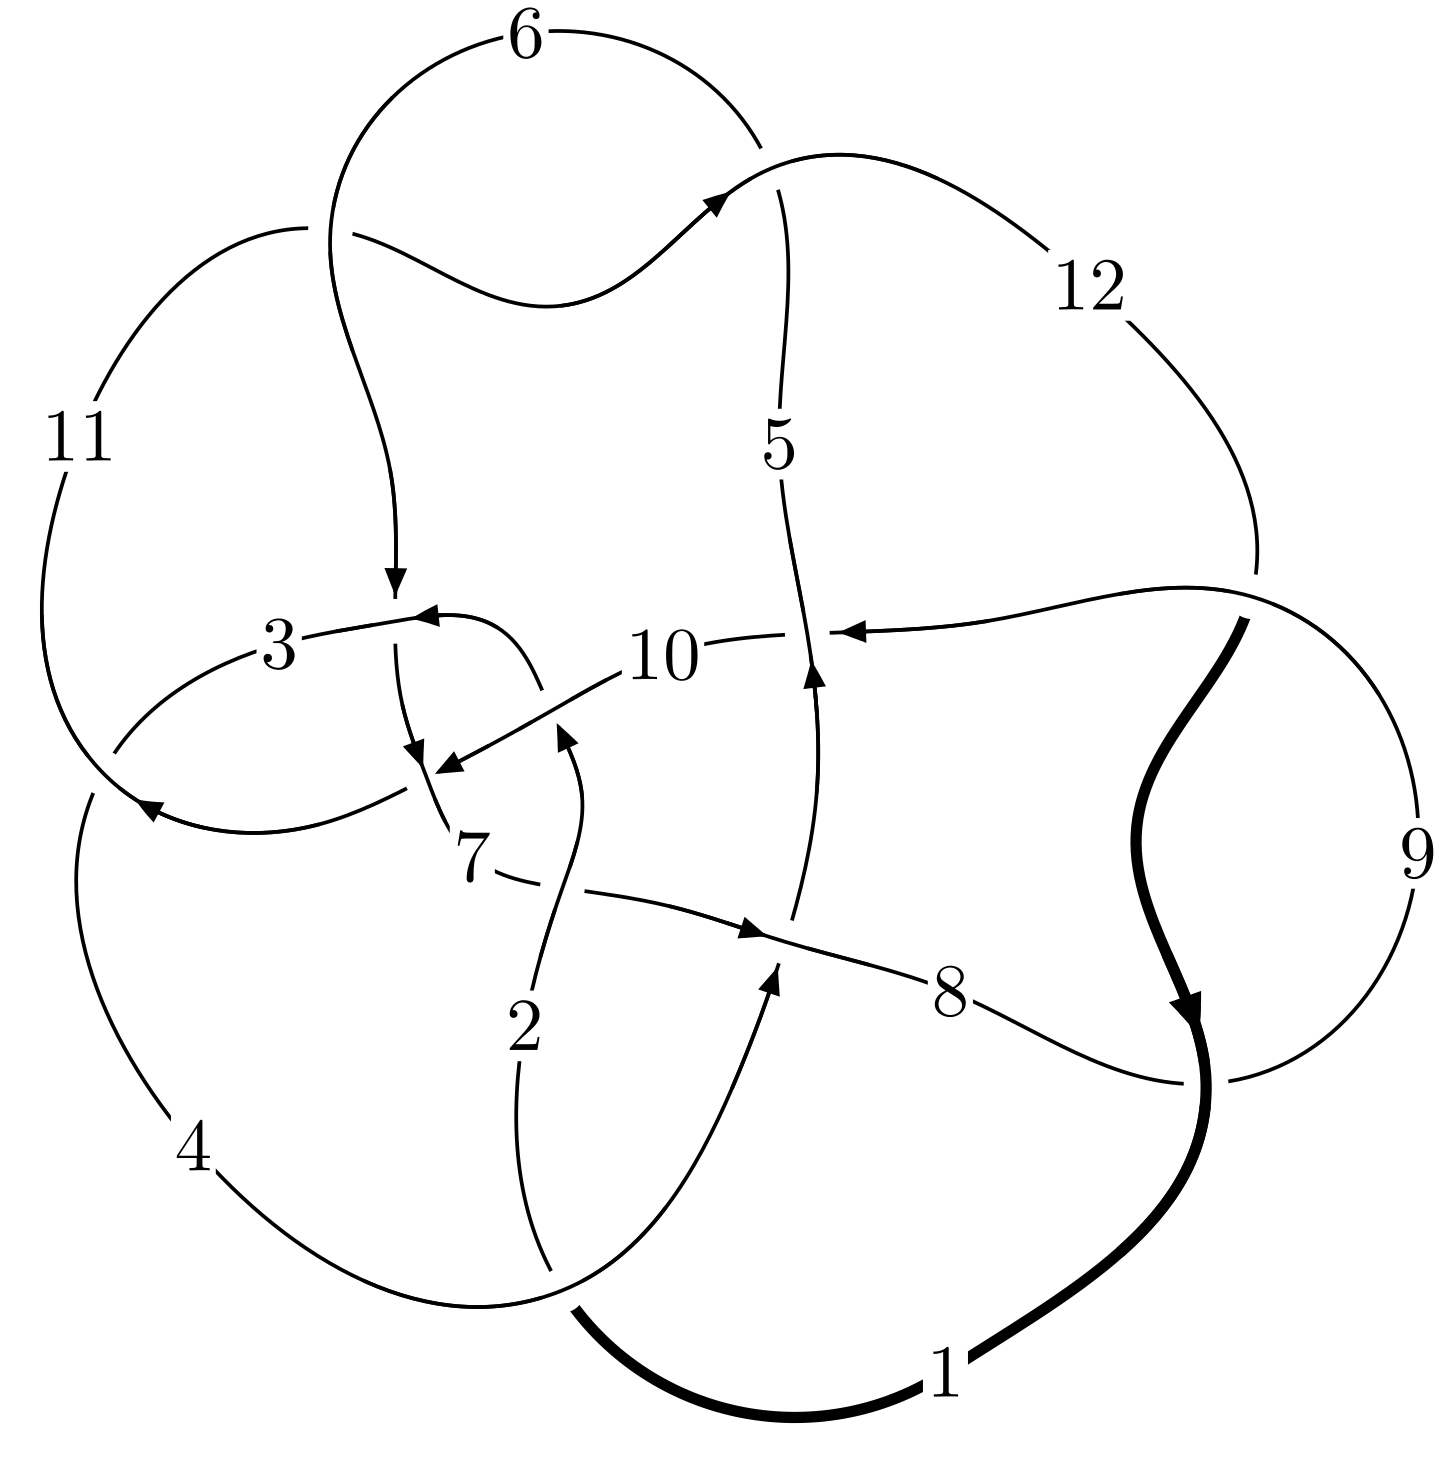
\includegraphics[width=112pt]{../../../GIT/diagram.site/Diagrams/png/1990_12a_1189.png}\\
\ \ \ A knot diagram\footnotemark}&
\allowdisplaybreaks
\textbf{Linearized knot diagam} \\
\cline{2-2}
 &
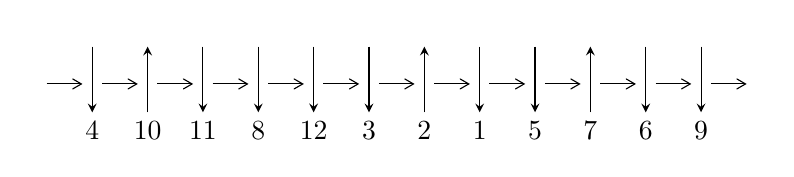
\begin{tikzpicture}[x=20pt, y=17pt]
	% nodes
	\node (C0) at (0, 0) {};
	\node (C1) at (1, 0) {};
	\node (C1U) at (1, +1) {};
	\node (C1D) at (1, -1) {4};

	\node (C2) at (2, 0) {};
	\node (C2U) at (2, +1) {};
	\node (C2D) at (2, -1) {10};

	\node (C3) at (3, 0) {};
	\node (C3U) at (3, +1) {};
	\node (C3D) at (3, -1) {11};

	\node (C4) at (4, 0) {};
	\node (C4U) at (4, +1) {};
	\node (C4D) at (4, -1) {8};

	\node (C5) at (5, 0) {};
	\node (C5U) at (5, +1) {};
	\node (C5D) at (5, -1) {12};

	\node (C6) at (6, 0) {};
	\node (C6U) at (6, +1) {};
	\node (C6D) at (6, -1) {3};

	\node (C7) at (7, 0) {};
	\node (C7U) at (7, +1) {};
	\node (C7D) at (7, -1) {2};

	\node (C8) at (8, 0) {};
	\node (C8U) at (8, +1) {};
	\node (C8D) at (8, -1) {1};

	\node (C9) at (9, 0) {};
	\node (C9U) at (9, +1) {};
	\node (C9D) at (9, -1) {5};

	\node (C10) at (10, 0) {};
	\node (C10U) at (10, +1) {};
	\node (C10D) at (10, -1) {7};

	\node (C11) at (11, 0) {};
	\node (C11U) at (11, +1) {};
	\node (C11D) at (11, -1) {6};

	\node (C12) at (12, 0) {};
	\node (C12U) at (12, +1) {};
	\node (C12D) at (12, -1) {9};
	\node (C13) at (13, 0) {};

	% arrows
	\draw[->,>={angle 60}]
	(C0) edge (C1) (C1) edge (C2) (C2) edge (C3) (C3) edge (C4) (C4) edge (C5) (C5) edge (C6) (C6) edge (C7) (C7) edge (C8) (C8) edge (C9) (C9) edge (C10) (C10) edge (C11) (C11) edge (C12) (C12) edge (C13) ;	\draw[->,>=stealth]
	(C1U) edge (C1D) (C2D) edge (C2U) (C3U) edge (C3D) (C4U) edge (C4D) (C5U) edge (C5D) (C6U) edge (C6D) (C7D) edge (C7U) (C8U) edge (C8D) (C9U) edge (C9D) (C10D) edge (C10U) (C11U) edge (C11D) (C12U) edge (C12D) ;
	\end{tikzpicture} \\
\hhline{~~} \\& 
\textbf{Solving Sequence} \\ \cline{2-2} 
 &
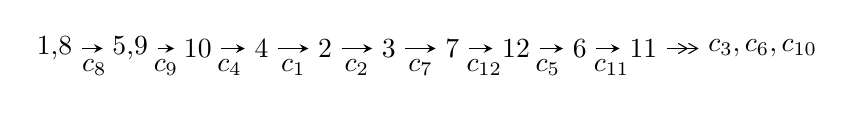
\begin{tikzpicture}[x=23pt, y=7pt]
	% node
	\node (A0) at (-1/8, 0) {1,8};
	\node (A1) at (17/16, 0) {5,9};
	\node (A2) at (17/8, 0) {10};
	\node (A3) at (25/8, 0) {4};
	\node (A4) at (33/8, 0) {2};
	\node (A5) at (41/8, 0) {3};
	\node (A6) at (49/8, 0) {7};
	\node (A7) at (57/8, 0) {12};
	\node (A8) at (65/8, 0) {6};
	\node (A9) at (73/8, 0) {11};
	\node (C1) at (1/2, -1) {$c_{8}$};
	\node (C2) at (13/8, -1) {$c_{9}$};
	\node (C3) at (21/8, -1) {$c_{4}$};
	\node (C4) at (29/8, -1) {$c_{1}$};
	\node (C5) at (37/8, -1) {$c_{2}$};
	\node (C6) at (45/8, -1) {$c_{7}$};
	\node (C7) at (53/8, -1) {$c_{12}$};
	\node (C8) at (61/8, -1) {$c_{5}$};
	\node (C9) at (69/8, -1) {$c_{11}$};
	\node (A10) at (11, 0) {$c_{3},c_{6},c_{10}$};

	% edge
	\draw[->,>=stealth]	
	(A0) edge (A1) (A1) edge (A2) (A2) edge (A3) (A3) edge (A4) (A4) edge (A5) (A5) edge (A6) (A6) edge (A7) (A7) edge (A8) (A8) edge (A9) ;
	\draw[->>,>={angle 60}]	
	(A9) edge (A10);
\end{tikzpicture} \\ 

\end{tabular} \\

\footnotetext{
The image of knot diagram is generated by the software ``\textbf{Draw programme}" developed by Andrew Bartholomew(\url{http://www.layer8.co.uk/maths/draw/index.htm\#Running-draw}), where we modified some parts for our purpose(\url{https://github.com/CATsTAILs/LinksPainter}).
}\phantom \\ \newline 
\centering \textbf{Ideals for irreducible components\footnotemark of $X_{\text{par}}$} 
 
\begin{align*}
I^u_{1}&=\langle 
-2.99880\times10^{1071} u^{178}-1.17856\times10^{1071} u^{177}+\cdots+3.13143\times10^{1072} b+1.70801\times10^{1074},\\
\phantom{I^u_{1}}&\phantom{= \langle  }8.49503\times10^{1072} u^{178}+4.90132\times10^{1073} u^{177}+\cdots+5.72157\times10^{1074} a-8.86831\times10^{1076},\\
\phantom{I^u_{1}}&\phantom{= \langle  }u^{179}+73 u^{177}+\cdots-29822 u-1279\rangle \\
I^u_{2}&=\langle 
-4.84269\times10^{37} u^{45}-1.67034\times10^{37} u^{44}+\cdots+5.81192\times10^{37} b+3.05918\times10^{38},\\
\phantom{I^u_{2}}&\phantom{= \langle  }1.74495\times10^{39} u^{45}+8.54988\times10^{38} u^{44}+\cdots+9.88026\times10^{38} a-3.34655\times10^{39},\;u^{46}+u^{45}+\cdots-15 u+17\rangle \\
\\
\end{align*}
\raggedright * 2 irreducible components of $\dim_{\mathbb{C}}=0$, with total 225 representations.\\
\footnotetext{All coefficients of polynomials are rational numbers. But the coefficients are sometimes approximated in decimal forms when there is not enough margin.}
\newpage
\renewcommand{\arraystretch}{1}
\centering \section*{I. $I^u_{1}= \langle -3.00\times10^{1071} u^{178}-1.18\times10^{1071} u^{177}+\cdots+3.13\times10^{1072} b+1.71\times10^{1074},\;8.50\times10^{1072} u^{178}+4.90\times10^{1073} u^{177}+\cdots+5.72\times10^{1074} a-8.87\times10^{1076},\;u^{179}+73 u^{177}+\cdots-29822 u-1279 \rangle$}
\flushleft \textbf{(i) Arc colorings}\\
\begin{tabular}{m{7pt} m{180pt} m{7pt} m{180pt} }
\flushright $a_{1}=$&$\begin{pmatrix}0\\u\end{pmatrix}$ \\
\flushright $a_{8}=$&$\begin{pmatrix}1\\0\end{pmatrix}$ \\
\flushright $a_{5}=$&$\begin{pmatrix}-0.0148474 u^{178}-0.0856639 u^{177}+\cdots+3341.59 u+154.998\\0.0957646 u^{178}+0.0376364 u^{177}+\cdots-1370.56 u-54.5443\end{pmatrix}$ \\
\flushright $a_{9}=$&$\begin{pmatrix}1\\u^2\end{pmatrix}$ \\
\flushright $a_{10}=$&$\begin{pmatrix}0.367758 u^{178}-0.176251 u^{177}+\cdots+2593.38 u+125.913\\-0.123380 u^{178}+0.116169 u^{177}+\cdots-1613.41 u-73.8663\end{pmatrix}$ \\
\flushright $a_{4}=$&$\begin{pmatrix}0.0809172 u^{178}-0.0480275 u^{177}+\cdots+1971.02 u+100.454\\0.0957646 u^{178}+0.0376364 u^{177}+\cdots-1370.56 u-54.5443\end{pmatrix}$ \\
\flushright $a_{2}=$&$\begin{pmatrix}0.0368696 u^{178}+0.211587 u^{177}+\cdots-4548.32 u-222.936\\0.0742994 u^{178}-0.0962500 u^{177}+\cdots+1794.54 u+81.1635\end{pmatrix}$ \\
\flushright $a_{3}=$&$\begin{pmatrix}-0.147173 u^{178}-0.293767 u^{177}+\cdots+6717.13 u+252.200\\0.110671 u^{178}+0.0320006 u^{177}+\cdots-894.570 u-33.8387\end{pmatrix}$ \\
\flushright $a_{7}=$&$\begin{pmatrix}-0.143066 u^{178}+0.119170 u^{177}+\cdots-2663.65 u-100.286\\0.0915930 u^{178}+0.0127491 u^{177}+\cdots-904.549 u-38.0392\end{pmatrix}$ \\
\flushright $a_{12}=$&$\begin{pmatrix}u\\u^3+u\end{pmatrix}$ \\
\flushright $a_{6}=$&$\begin{pmatrix}0.0668388 u^{178}-0.0538365 u^{177}+\cdots+2403.04 u+118.319\\0.0567337 u^{178}+0.0421875 u^{177}+\cdots-1255.47 u-50.5159\end{pmatrix}$ \\
\flushright $a_{11}=$&$\begin{pmatrix}0.122140 u^{178}+0.0869151 u^{177}+\cdots-1281.44 u-18.3700\\0.0298642 u^{178}+0.0769529 u^{177}+\cdots-1595.47 u-68.8104\end{pmatrix}$\\&\end{tabular}
\flushleft \textbf{(ii) Obstruction class $= -1$}\\~\\
\flushleft \textbf{(iii) Cusp Shapes $= 0.555247 u^{178}+1.26086 u^{177}+\cdots-26877.2 u-1134.04$}\\~\\
\newpage\renewcommand{\arraystretch}{1}
\flushleft \textbf{(iv) u-Polynomials at the component}\newline \\
\begin{tabular}{m{50pt}|m{274pt}}
Crossings & \hspace{64pt}u-Polynomials at each crossing \\
\hline $$\begin{aligned}c_{1}\end{aligned}$$&$\begin{aligned}
&u^{179}+3 u^{178}+\cdots+5846731 u+1313576
\end{aligned}$\\
\hline $$\begin{aligned}c_{2}\end{aligned}$$&$\begin{aligned}
&u^{179}+4 u^{178}+\cdots+36391 u+11019
\end{aligned}$\\
\hline $$\begin{aligned}c_{3}\end{aligned}$$&$\begin{aligned}
&u^{179}+25 u^{177}+\cdots-341620 u+43669
\end{aligned}$\\
\hline $$\begin{aligned}c_{4}\end{aligned}$$&$\begin{aligned}
&u^{179}- u^{178}+\cdots+5 u+1
\end{aligned}$\\
\hline $$\begin{aligned}c_{5},c_{11}\end{aligned}$$&$\begin{aligned}
&u^{179}- u^{178}+\cdots-21986697 u+1238227
\end{aligned}$\\
\hline $$\begin{aligned}c_{6}\end{aligned}$$&$\begin{aligned}
&u^{179}-2 u^{178}+\cdots-146753 u+4679
\end{aligned}$\\
\hline $$\begin{aligned}c_{7}\end{aligned}$$&$\begin{aligned}
&u^{179}-2 u^{178}+\cdots+20083300 u+2036725
\end{aligned}$\\
\hline $$\begin{aligned}c_{8},c_{12}\end{aligned}$$&$\begin{aligned}
&u^{179}+73 u^{177}+\cdots-29822 u+1279
\end{aligned}$\\
\hline $$\begin{aligned}c_{9}\end{aligned}$$&$\begin{aligned}
&u^{179}- u^{178}+\cdots-191134085123 u+17016804162
\end{aligned}$\\
\hline $$\begin{aligned}c_{10}\end{aligned}$$&$\begin{aligned}
&u^{179}-7 u^{178}+\cdots+57 u+4
\end{aligned}$\\
\hline
\end{tabular}\\~\\
\newpage\renewcommand{\arraystretch}{1}
\flushleft \textbf{(v) Riley Polynomials at the component}\newline \\
\begin{tabular}{m{50pt}|m{274pt}}
Crossings & \hspace{64pt}Riley Polynomials at each crossing \\
\hline $$\begin{aligned}c_{1}\end{aligned}$$&$\begin{aligned}
&y^{179}+29 y^{178}+\cdots+37780934306137 y-1725481907776
\end{aligned}$\\
\hline $$\begin{aligned}c_{2}\end{aligned}$$&$\begin{aligned}
&y^{179}+8 y^{178}+\cdots+5723288023 y-121418361
\end{aligned}$\\
\hline $$\begin{aligned}c_{3}\end{aligned}$$&$\begin{aligned}
&y^{179}+50 y^{178}+\cdots-139738921270 y-1906981561
\end{aligned}$\\
\hline $$\begin{aligned}c_{4}\end{aligned}$$&$\begin{aligned}
&y^{179}+17 y^{178}+\cdots-429 y-1
\end{aligned}$\\
\hline $$\begin{aligned}c_{5},c_{11}\end{aligned}$$&$\begin{aligned}
&y^{179}+151 y^{178}+\cdots+108984338877843 y-1533206103529
\end{aligned}$\\
\hline $$\begin{aligned}c_{6}\end{aligned}$$&$\begin{aligned}
&y^{179}+40 y^{178}+\cdots+4864670035 y-21893041
\end{aligned}$\\
\hline $$\begin{aligned}c_{7}\end{aligned}$$&$\begin{aligned}
&y^{179}+62 y^{178}+\cdots-224749595737250 y-4148248725625
\end{aligned}$\\
\hline $$\begin{aligned}c_{8},c_{12}\end{aligned}$$&$\begin{aligned}
&y^{179}+146 y^{178}+\cdots+119524142 y-1635841
\end{aligned}$\\
\hline $$\begin{aligned}c_{9}\end{aligned}$$&$\begin{aligned}
&y^{179}+87 y^{178}+\cdots-4.54\times10^{21} y-2.90\times10^{20}
\end{aligned}$\\
\hline $$\begin{aligned}c_{10}\end{aligned}$$&$\begin{aligned}
&y^{179}+13 y^{178}+\cdots-615 y-16
\end{aligned}$\\
\hline
\end{tabular}\\~\\
\newpage\flushleft \textbf{(vi) Complex Volumes and Cusp Shapes}
$$\begin{array}{c|c|c}  
\text{Solutions to }I^u_{1}& \I (\text{vol} + \sqrt{-1}CS) & \text{Cusp shape}\\
 \hline 
\begin{aligned}
u &= \phantom{-}0.998280 + 0.070214 I \\
a &= \phantom{-}0.204320 + 0.216189 I \\
b &= \phantom{-}0.828235 + 0.365604 I\end{aligned}
 & -3.69915 - 2.13626 I & \phantom{-0.000000 } 0 \\ \hline\begin{aligned}
u &= \phantom{-}0.998280 - 0.070214 I \\
a &= \phantom{-}0.204320 - 0.216189 I \\
b &= \phantom{-}0.828235 - 0.365604 I\end{aligned}
 & -3.69915 + 2.13626 I & \phantom{-0.000000 } 0 \\ \hline\begin{aligned}
u &= -0.203391 + 0.977006 I \\
a &= -0.75818 + 1.94321 I \\
b &= \phantom{-}0.328121 - 0.205351 I\end{aligned}
 & -0.76644 + 6.70484 I & \phantom{-0.000000 } 0 \\ \hline\begin{aligned}
u &= -0.203391 - 0.977006 I \\
a &= -0.75818 - 1.94321 I \\
b &= \phantom{-}0.328121 + 0.205351 I\end{aligned}
 & -0.76644 - 6.70484 I & \phantom{-0.000000 } 0 \\ \hline\begin{aligned}
u &= \phantom{-}0.625829 + 0.796750 I \\
a &= \phantom{-}1.162870 - 0.699282 I \\
b &= \phantom{-}0.657821 - 0.037010 I\end{aligned}
 & -0.14305 - 2.48684 I & \phantom{-0.000000 } 0 \\ \hline\begin{aligned}
u &= \phantom{-}0.625829 - 0.796750 I \\
a &= \phantom{-}1.162870 + 0.699282 I \\
b &= \phantom{-}0.657821 + 0.037010 I\end{aligned}
 & -0.14305 + 2.48684 I & \phantom{-0.000000 } 0 \\ \hline\begin{aligned}
u &= -0.844809 + 0.481059 I \\
a &= -0.112688 - 0.317881 I \\
b &= -1.095970 + 0.680098 I\end{aligned}
 & \phantom{-}1.42232 + 5.50398 I & \phantom{-0.000000 } 0 \\ \hline\begin{aligned}
u &= -0.844809 - 0.481059 I \\
a &= -0.112688 + 0.317881 I \\
b &= -1.095970 - 0.680098 I\end{aligned}
 & \phantom{-}1.42232 - 5.50398 I & \phantom{-0.000000 } 0 \\ \hline\begin{aligned}
u &= -0.943635 + 0.028748 I \\
a &= -0.104136 + 0.225943 I \\
b &= \phantom{-}0.923089 + 0.734300 I\end{aligned}
 & -2.98651 - 9.84844 I & \phantom{-0.000000 } 0 \\ \hline\begin{aligned}
u &= -0.943635 - 0.028748 I \\
a &= -0.104136 - 0.225943 I \\
b &= \phantom{-}0.923089 - 0.734300 I\end{aligned}
 & -2.98651 + 9.84844 I & \phantom{-0.000000 } 0\\
 \hline 
 \end{array}$$\newpage$$\begin{array}{c|c|c}  
\text{Solutions to }I^u_{1}& \I (\text{vol} + \sqrt{-1}CS) & \text{Cusp shape}\\
 \hline 
\begin{aligned}
u &= \phantom{-}0.290224 + 1.030880 I \\
a &= -0.37203 + 2.63842 I \\
b &= -0.258940 - 0.074070 I\end{aligned}
 & \phantom{-}4.41541 - 10.41770 I & \phantom{-0.000000 } 0 \\ \hline\begin{aligned}
u &= \phantom{-}0.290224 - 1.030880 I \\
a &= -0.37203 - 2.63842 I \\
b &= -0.258940 + 0.074070 I\end{aligned}
 & \phantom{-}4.41541 + 10.41770 I & \phantom{-0.000000 } 0 \\ \hline\begin{aligned}
u &= -0.138430 + 1.078030 I \\
a &= -0.06314 - 1.47184 I \\
b &= -1.17336 + 1.00087 I\end{aligned}
 & \phantom{-}1.99950 + 3.54359 I & \phantom{-0.000000 } 0 \\ \hline\begin{aligned}
u &= -0.138430 - 1.078030 I \\
a &= -0.06314 + 1.47184 I \\
b &= -1.17336 - 1.00087 I\end{aligned}
 & \phantom{-}1.99950 - 3.54359 I & \phantom{-0.000000 } 0 \\ \hline\begin{aligned}
u &= -0.372417 + 0.815265 I \\
a &= -0.519155 - 0.487549 I \\
b &= -1.095430 + 0.156344 I\end{aligned}
 & -1.97343 + 2.95696 I & \phantom{-0.000000 } 0 \\ \hline\begin{aligned}
u &= -0.372417 - 0.815265 I \\
a &= -0.519155 + 0.487549 I \\
b &= -1.095430 - 0.156344 I\end{aligned}
 & -1.97343 - 2.95696 I & \phantom{-0.000000 } 0 \\ \hline\begin{aligned}
u &= \phantom{-}0.890167 + 0.076860 I \\
a &= \phantom{-}0.521445 + 0.218787 I \\
b &= \phantom{-}0.885195 - 0.800858 I\end{aligned}
 & -0.71037 + 2.97355 I & \phantom{-0.000000 } 0 \\ \hline\begin{aligned}
u &= \phantom{-}0.890167 - 0.076860 I \\
a &= \phantom{-}0.521445 - 0.218787 I \\
b &= \phantom{-}0.885195 + 0.800858 I\end{aligned}
 & -0.71037 - 2.97355 I & \phantom{-0.000000 } 0 \\ \hline\begin{aligned}
u &= -0.782405 + 0.424071 I \\
a &= \phantom{-}0.480978 - 0.907026 I \\
b &= -0.808448 - 0.228556 I\end{aligned}
 & \phantom{-}1.179990 - 0.329076 I & \phantom{-0.000000 } 0 \\ \hline\begin{aligned}
u &= -0.782405 - 0.424071 I \\
a &= \phantom{-}0.480978 + 0.907026 I \\
b &= -0.808448 + 0.228556 I\end{aligned}
 & \phantom{-}1.179990 + 0.329076 I & \phantom{-0.000000 } 0\\
 \hline 
 \end{array}$$\newpage$$\begin{array}{c|c|c}  
\text{Solutions to }I^u_{1}& \I (\text{vol} + \sqrt{-1}CS) & \text{Cusp shape}\\
 \hline 
\begin{aligned}
u &= \phantom{-}0.006310 + 1.112580 I \\
a &= \phantom{-}0.308509 + 1.086530 I \\
b &= \phantom{-}0.206645 - 0.801155 I\end{aligned}
 & \phantom{-}2.54569 - 1.54986 I & \phantom{-0.000000 } 0 \\ \hline\begin{aligned}
u &= \phantom{-}0.006310 - 1.112580 I \\
a &= \phantom{-}0.308509 - 1.086530 I \\
b &= \phantom{-}0.206645 + 0.801155 I\end{aligned}
 & \phantom{-}2.54569 + 1.54986 I & \phantom{-0.000000 } 0 \\ \hline\begin{aligned}
u &= \phantom{-}0.216435 + 1.099000 I \\
a &= \phantom{-}0.50639 + 2.07951 I \\
b &= -1.40103 - 1.83182 I\end{aligned}
 & \phantom{-}1.29206 - 5.74333 I & \phantom{-0.000000 } 0 \\ \hline\begin{aligned}
u &= \phantom{-}0.216435 - 1.099000 I \\
a &= \phantom{-}0.50639 - 2.07951 I \\
b &= -1.40103 + 1.83182 I\end{aligned}
 & \phantom{-}1.29206 + 5.74333 I & \phantom{-0.000000 } 0 \\ \hline\begin{aligned}
u &= -1.088110 + 0.266292 I \\
a &= \phantom{-}0.006643 + 0.193021 I \\
b &= \phantom{-}0.847155 - 0.701964 I\end{aligned}
 & \phantom{-}3.54219 + 7.00380 I & \phantom{-0.000000 } 0 \\ \hline\begin{aligned}
u &= -1.088110 - 0.266292 I \\
a &= \phantom{-}0.006643 - 0.193021 I \\
b &= \phantom{-}0.847155 + 0.701964 I\end{aligned}
 & \phantom{-}3.54219 - 7.00380 I & \phantom{-0.000000 } 0 \\ \hline\begin{aligned}
u &= -0.018113 + 1.129000 I \\
a &= -0.613434 - 0.794980 I \\
b &= -1.105060 + 0.461681 I\end{aligned}
 & \phantom{-}2.53352 + 3.03096 I & \phantom{-0.000000 } 0 \\ \hline\begin{aligned}
u &= -0.018113 - 1.129000 I \\
a &= -0.613434 + 0.794980 I \\
b &= -1.105060 - 0.461681 I\end{aligned}
 & \phantom{-}2.53352 - 3.03096 I & \phantom{-0.000000 } 0 \\ \hline\begin{aligned}
u &= -0.888857 + 0.699512 I \\
a &= -0.960511 - 0.010202 I \\
b &= -0.564599 + 0.295250 I\end{aligned}
 & \phantom{-}1.74555 + 3.46899 I & \phantom{-0.000000 } 0 \\ \hline\begin{aligned}
u &= -0.888857 - 0.699512 I \\
a &= -0.960511 + 0.010202 I \\
b &= -0.564599 - 0.295250 I\end{aligned}
 & \phantom{-}1.74555 - 3.46899 I & \phantom{-0.000000 } 0\\
 \hline 
 \end{array}$$\newpage$$\begin{array}{c|c|c}  
\text{Solutions to }I^u_{1}& \I (\text{vol} + \sqrt{-1}CS) & \text{Cusp shape}\\
 \hline 
\begin{aligned}
u &= \phantom{-}0.074897 + 1.144160 I \\
a &= -0.01616 - 2.27465 I \\
b &= \phantom{-}0.49613 + 2.17691 I\end{aligned}
 & \phantom{-}2.28209 + 3.73578 I & \phantom{-0.000000 } 0 \\ \hline\begin{aligned}
u &= \phantom{-}0.074897 - 1.144160 I \\
a &= -0.01616 + 2.27465 I \\
b &= \phantom{-}0.49613 - 2.17691 I\end{aligned}
 & \phantom{-}2.28209 - 3.73578 I & \phantom{-0.000000 } 0 \\ \hline\begin{aligned}
u &= -0.194250 + 1.155580 I \\
a &= \phantom{-}0.42104 - 1.89422 I \\
b &= -1.10300 + 1.17132 I\end{aligned}
 & -0.00825 + 3.71965 I & \phantom{-0.000000 } 0 \\ \hline\begin{aligned}
u &= -0.194250 - 1.155580 I \\
a &= \phantom{-}0.42104 + 1.89422 I \\
b &= -1.10300 - 1.17132 I\end{aligned}
 & -0.00825 - 3.71965 I & \phantom{-0.000000 } 0 \\ \hline\begin{aligned}
u &= \phantom{-}0.826046 + 0.000663 I \\
a &= -0.023868 + 0.148020 I \\
b &= -0.994024 - 0.482209 I\end{aligned}
 & -3.45729 - 0.07241 I & \phantom{-0.000000 } 0 \\ \hline\begin{aligned}
u &= \phantom{-}0.826046 - 0.000663 I \\
a &= -0.023868 - 0.148020 I \\
b &= -0.994024 + 0.482209 I\end{aligned}
 & -3.45729 + 0.07241 I & \phantom{-0.000000 } 0 \\ \hline\begin{aligned}
u &= -1.159600 + 0.191919 I \\
a &= \phantom{-}0.121254 + 0.287426 I \\
b &= \phantom{-}0.413498 - 0.567229 I\end{aligned}
 & \phantom{-}4.65237 + 1.13699 I & \phantom{-0.000000 } 0 \\ \hline\begin{aligned}
u &= -1.159600 - 0.191919 I \\
a &= \phantom{-}0.121254 - 0.287426 I \\
b &= \phantom{-}0.413498 + 0.567229 I\end{aligned}
 & \phantom{-}4.65237 - 1.13699 I & \phantom{-0.000000 } 0 \\ \hline\begin{aligned}
u &= -0.145521 + 0.809666 I \\
a &= \phantom{-}1.42063 + 0.66833 I \\
b &= -0.369397 - 0.675864 I\end{aligned}
 & \phantom{-}1.19068 - 2.43159 I & \phantom{-0.000000 } 0 \\ \hline\begin{aligned}
u &= -0.145521 - 0.809666 I \\
a &= \phantom{-}1.42063 - 0.66833 I \\
b &= -0.369397 + 0.675864 I\end{aligned}
 & \phantom{-}1.19068 + 2.43159 I & \phantom{-0.000000 } 0\\
 \hline 
 \end{array}$$\newpage$$\begin{array}{c|c|c}  
\text{Solutions to }I^u_{1}& \I (\text{vol} + \sqrt{-1}CS) & \text{Cusp shape}\\
 \hline 
\begin{aligned}
u &= -0.210116 + 1.160010 I \\
a &= -0.82802 + 1.54617 I \\
b &= \phantom{-}1.45093 - 1.05280 I\end{aligned}
 & -0.00427 - 2.20221 I & \phantom{-0.000000 } 0 \\ \hline\begin{aligned}
u &= -0.210116 - 1.160010 I \\
a &= -0.82802 - 1.54617 I \\
b &= \phantom{-}1.45093 + 1.05280 I\end{aligned}
 & -0.00427 + 2.20221 I & \phantom{-0.000000 } 0 \\ \hline\begin{aligned}
u &= \phantom{-}0.023813 + 1.191270 I \\
a &= \phantom{-}1.06050 + 2.25117 I \\
b &= \phantom{-}0.509622 - 0.755946 I\end{aligned}
 & \phantom{-}6.40961 + 8.79257 I & \phantom{-0.000000 } 0 \\ \hline\begin{aligned}
u &= \phantom{-}0.023813 - 1.191270 I \\
a &= \phantom{-}1.06050 - 2.25117 I \\
b &= \phantom{-}0.509622 + 0.755946 I\end{aligned}
 & \phantom{-}6.40961 - 8.79257 I & \phantom{-0.000000 } 0 \\ \hline\begin{aligned}
u &= \phantom{-}0.017408 + 1.204010 I \\
a &= -0.422614 - 1.333090 I \\
b &= \phantom{-}1.52675 + 0.83299 I\end{aligned}
 & \phantom{-}6.26412 - 2.13728 I & \phantom{-0.000000 } 0 \\ \hline\begin{aligned}
u &= \phantom{-}0.017408 - 1.204010 I \\
a &= -0.422614 + 1.333090 I \\
b &= \phantom{-}1.52675 - 0.83299 I\end{aligned}
 & \phantom{-}6.26412 + 2.13728 I & \phantom{-0.000000 } 0 \\ \hline\begin{aligned}
u &= \phantom{-}0.621296 + 0.497334 I \\
a &= \phantom{-}0.685258 + 0.198504 I \\
b &= \phantom{-}0.909730 + 0.446928 I\end{aligned}
 & -1.98136 - 4.27856 I & \phantom{-0.000000 } 0 \\ \hline\begin{aligned}
u &= \phantom{-}0.621296 - 0.497334 I \\
a &= \phantom{-}0.685258 - 0.198504 I \\
b &= \phantom{-}0.909730 - 0.446928 I\end{aligned}
 & -1.98136 + 4.27856 I & \phantom{-0.000000 } 0 \\ \hline\begin{aligned}
u &= -0.779323 + 0.133995 I \\
a &= -0.027444 - 0.585367 I \\
b &= -0.862957 - 0.735222 I\end{aligned}
 & -2.54274 - 3.40144 I & \phantom{-0.000000 } 0 \\ \hline\begin{aligned}
u &= -0.779323 - 0.133995 I \\
a &= -0.027444 + 0.585367 I \\
b &= -0.862957 + 0.735222 I\end{aligned}
 & -2.54274 + 3.40144 I & \phantom{-0.000000 } 0\\
 \hline 
 \end{array}$$\newpage$$\begin{array}{c|c|c}  
\text{Solutions to }I^u_{1}& \I (\text{vol} + \sqrt{-1}CS) & \text{Cusp shape}\\
 \hline 
\begin{aligned}
u &= \phantom{-}0.785809 + 0.069975 I \\
a &= \phantom{-}0.410376 + 0.362473 I \\
b &= -0.775894 + 0.557055 I\end{aligned}
 & -0.678724 + 1.153220 I & \phantom{-0.000000 } 0 \\ \hline\begin{aligned}
u &= \phantom{-}0.785809 - 0.069975 I \\
a &= \phantom{-}0.410376 - 0.362473 I \\
b &= -0.775894 - 0.557055 I\end{aligned}
 & -0.678724 - 1.153220 I & \phantom{-0.000000 } 0 \\ \hline\begin{aligned}
u &= \phantom{-}0.631661 + 0.470397 I \\
a &= -1.64955 - 0.45249 I \\
b &= -0.822070 + 0.053916 I\end{aligned}
 & \phantom{-}2.89936 + 6.75098 I & \phantom{-0.000000 } 0 \\ \hline\begin{aligned}
u &= \phantom{-}0.631661 - 0.470397 I \\
a &= -1.64955 + 0.45249 I \\
b &= -0.822070 - 0.053916 I\end{aligned}
 & \phantom{-}2.89936 - 6.75098 I & \phantom{-0.000000 } 0 \\ \hline\begin{aligned}
u &= \phantom{-}0.584502 + 0.527544 I \\
a &= \phantom{-}1.359900 + 0.125024 I \\
b &= -0.949435 + 0.827786 I\end{aligned}
 & -0.38675 + 2.66722 I & \phantom{-0.000000 } 0 \\ \hline\begin{aligned}
u &= \phantom{-}0.584502 - 0.527544 I \\
a &= \phantom{-}1.359900 - 0.125024 I \\
b &= -0.949435 - 0.827786 I\end{aligned}
 & -0.38675 - 2.66722 I & \phantom{-0.000000 } 0 \\ \hline\begin{aligned}
u &= -0.383802 + 1.150470 I \\
a &= -0.47772 - 1.56105 I \\
b &= -0.39683 + 1.50899 I\end{aligned}
 & \phantom{-}4.23779 + 6.18551 I & \phantom{-0.000000 } 0 \\ \hline\begin{aligned}
u &= -0.383802 - 1.150470 I \\
a &= -0.47772 + 1.56105 I \\
b &= -0.39683 - 1.50899 I\end{aligned}
 & \phantom{-}4.23779 - 6.18551 I & \phantom{-0.000000 } 0 \\ \hline\begin{aligned}
u &= \phantom{-}1.187980 + 0.246415 I \\
a &= -0.100408 + 0.159658 I \\
b &= -0.904353 - 0.768967 I\end{aligned}
 & \phantom{-}2.3271 - 14.9993 I & \phantom{-0.000000 } 0 \\ \hline\begin{aligned}
u &= \phantom{-}1.187980 - 0.246415 I \\
a &= -0.100408 - 0.159658 I \\
b &= -0.904353 + 0.768967 I\end{aligned}
 & \phantom{-}2.3271 + 14.9993 I & \phantom{-0.000000 } 0\\
 \hline 
 \end{array}$$\newpage$$\begin{array}{c|c|c}  
\text{Solutions to }I^u_{1}& \I (\text{vol} + \sqrt{-1}CS) & \text{Cusp shape}\\
 \hline 
\begin{aligned}
u &= \phantom{-}0.249436 + 1.191870 I \\
a &= -0.77682 + 1.80243 I \\
b &= -0.612784 - 0.851292 I\end{aligned}
 & \phantom{-}2.94167 - 7.34369 I & \phantom{-0.000000 } 0 \\ \hline\begin{aligned}
u &= \phantom{-}0.249436 - 1.191870 I \\
a &= -0.77682 - 1.80243 I \\
b &= -0.612784 + 0.851292 I\end{aligned}
 & \phantom{-}2.94167 + 7.34369 I & \phantom{-0.000000 } 0 \\ \hline\begin{aligned}
u &= \phantom{-}0.483159 + 1.124930 I \\
a &= \phantom{-}0.179283 - 0.941424 I \\
b &= \phantom{-}0.413858 + 0.268609 I\end{aligned}
 & -0.52339 - 3.21299 I & \phantom{-0.000000 } 0 \\ \hline\begin{aligned}
u &= \phantom{-}0.483159 - 1.124930 I \\
a &= \phantom{-}0.179283 + 0.941424 I \\
b &= \phantom{-}0.413858 - 0.268609 I\end{aligned}
 & -0.52339 + 3.21299 I & \phantom{-0.000000 } 0 \\ \hline\begin{aligned}
u &= -0.194489 + 0.748093 I \\
a &= \phantom{-}0.32961 - 1.62739 I \\
b &= -0.448962 - 0.009640 I\end{aligned}
 & -1.97376 - 0.12088 I & \phantom{-0.000000 } 0 \\ \hline\begin{aligned}
u &= -0.194489 - 0.748093 I \\
a &= \phantom{-}0.32961 + 1.62739 I \\
b &= -0.448962 + 0.009640 I\end{aligned}
 & -1.97376 + 0.12088 I & \phantom{-0.000000 } 0 \\ \hline\begin{aligned}
u &= -0.113811 + 1.225650 I \\
a &= \phantom{-}0.04586 - 2.49718 I \\
b &= \phantom{-}0.325548 + 1.375430 I\end{aligned}
 & \phantom{-}7.75387 + 2.04834 I & \phantom{-0.000000 } 0 \\ \hline\begin{aligned}
u &= -0.113811 - 1.225650 I \\
a &= \phantom{-}0.04586 + 2.49718 I \\
b &= \phantom{-}0.325548 - 1.375430 I\end{aligned}
 & \phantom{-}7.75387 - 2.04834 I & \phantom{-0.000000 } 0 \\ \hline\begin{aligned}
u &= -0.107242 + 1.227000 I \\
a &= -0.91817 - 1.76488 I \\
b &= \phantom{-}1.35755 + 1.58563 I\end{aligned}
 & \phantom{-}8.50074 + 3.17466 I & \phantom{-0.000000 } 0 \\ \hline\begin{aligned}
u &= -0.107242 - 1.227000 I \\
a &= -0.91817 + 1.76488 I \\
b &= \phantom{-}1.35755 - 1.58563 I\end{aligned}
 & \phantom{-}8.50074 - 3.17466 I & \phantom{-0.000000 } 0\\
 \hline 
 \end{array}$$\newpage$$\begin{array}{c|c|c}  
\text{Solutions to }I^u_{1}& \I (\text{vol} + \sqrt{-1}CS) & \text{Cusp shape}\\
 \hline 
\begin{aligned}
u &= -0.635049 + 1.063310 I \\
a &= -0.377986 - 0.663571 I \\
b &= \phantom{-}0.0093248 - 0.0686050 I\end{aligned}
 & \phantom{-}2.92788 + 2.78840 I & \phantom{-0.000000 } 0 \\ \hline\begin{aligned}
u &= -0.635049 - 1.063310 I \\
a &= -0.377986 + 0.663571 I \\
b &= \phantom{-}0.0093248 + 0.0686050 I\end{aligned}
 & \phantom{-}2.92788 - 2.78840 I & \phantom{-0.000000 } 0 \\ \hline\begin{aligned}
u &= \phantom{-}0.022331 + 1.251760 I \\
a &= -0.875358 + 0.965655 I \\
b &= \phantom{-}1.92228 - 1.02277 I\end{aligned}
 & \phantom{-}7.95765 - 3.75761 I & \phantom{-0.000000 } 0 \\ \hline\begin{aligned}
u &= \phantom{-}0.022331 - 1.251760 I \\
a &= -0.875358 - 0.965655 I \\
b &= \phantom{-}1.92228 + 1.02277 I\end{aligned}
 & \phantom{-}7.95765 + 3.75761 I & \phantom{-0.000000 } 0 \\ \hline\begin{aligned}
u &= -0.114488 + 1.248380 I \\
a &= -0.20368 + 2.39590 I \\
b &= -0.095086 - 1.109260 I\end{aligned}
 & \phantom{-}8.82921 - 0.06805 I & \phantom{-0.000000 } 0 \\ \hline\begin{aligned}
u &= -0.114488 - 1.248380 I \\
a &= -0.20368 - 2.39590 I \\
b &= -0.095086 + 1.109260 I\end{aligned}
 & \phantom{-}8.82921 + 0.06805 I & \phantom{-0.000000 } 0 \\ \hline\begin{aligned}
u &= \phantom{-}0.365143 + 1.208030 I \\
a &= \phantom{-}0.589842 - 0.246454 I \\
b &= \phantom{-}0.257695 + 0.328767 I\end{aligned}
 & \phantom{-}3.20830 - 2.72130 I & \phantom{-0.000000 } 0 \\ \hline\begin{aligned}
u &= \phantom{-}0.365143 - 1.208030 I \\
a &= \phantom{-}0.589842 + 0.246454 I \\
b &= \phantom{-}0.257695 - 0.328767 I\end{aligned}
 & \phantom{-}3.20830 + 2.72130 I & \phantom{-0.000000 } 0 \\ \hline\begin{aligned}
u &= -0.185617 + 1.251140 I \\
a &= -0.774356 - 0.613941 I \\
b &= \phantom{-}1.43282 + 0.51073 I\end{aligned}
 & \phantom{-}7.71028 + 0.74474 I & \phantom{-0.000000 } 0 \\ \hline\begin{aligned}
u &= -0.185617 - 1.251140 I \\
a &= -0.774356 + 0.613941 I \\
b &= \phantom{-}1.43282 - 0.51073 I\end{aligned}
 & \phantom{-}7.71028 - 0.74474 I & \phantom{-0.000000 } 0\\
 \hline 
 \end{array}$$\newpage$$\begin{array}{c|c|c}  
\text{Solutions to }I^u_{1}& \I (\text{vol} + \sqrt{-1}CS) & \text{Cusp shape}\\
 \hline 
\begin{aligned}
u &= -0.103702 + 1.277190 I \\
a &= -1.003770 + 0.287151 I \\
b &= -0.417110 + 0.048559 I\end{aligned}
 & \phantom{-}8.51114 + 4.80921 I & \phantom{-0.000000 } 0 \\ \hline\begin{aligned}
u &= -0.103702 - 1.277190 I \\
a &= -1.003770 - 0.287151 I \\
b &= -0.417110 - 0.048559 I\end{aligned}
 & \phantom{-}8.51114 - 4.80921 I & \phantom{-0.000000 } 0 \\ \hline\begin{aligned}
u &= -0.170448 + 1.278170 I \\
a &= -0.389770 + 1.297600 I \\
b &= -0.330182 - 0.644056 I\end{aligned}
 & \phantom{-}8.25077 + 4.62962 I & \phantom{-0.000000 } 0 \\ \hline\begin{aligned}
u &= -0.170448 - 1.278170 I \\
a &= -0.389770 - 1.297600 I \\
b &= -0.330182 + 0.644056 I\end{aligned}
 & \phantom{-}8.25077 - 4.62962 I & \phantom{-0.000000 } 0 \\ \hline\begin{aligned}
u &= \phantom{-}0.397944 + 1.230100 I \\
a &= \phantom{-}0.23725 + 1.58258 I \\
b &= -1.04418 - 1.34440 I\end{aligned}
 & \phantom{-}2.86710 - 5.49138 I & \phantom{-0.000000 } 0 \\ \hline\begin{aligned}
u &= \phantom{-}0.397944 - 1.230100 I \\
a &= \phantom{-}0.23725 - 1.58258 I \\
b &= -1.04418 + 1.34440 I\end{aligned}
 & \phantom{-}2.86710 + 5.49138 I & \phantom{-0.000000 } 0 \\ \hline\begin{aligned}
u &= \phantom{-}0.446695 + 0.547985 I \\
a &= \phantom{-}0.261230 - 1.037440 I \\
b &= \phantom{-}0.096193 - 0.330347 I\end{aligned}
 & -1.65076 + 0.00178 I & \phantom{-0.000000 } 0 \\ \hline\begin{aligned}
u &= \phantom{-}0.446695 - 0.547985 I \\
a &= \phantom{-}0.261230 + 1.037440 I \\
b &= \phantom{-}0.096193 + 0.330347 I\end{aligned}
 & -1.65076 - 0.00178 I & \phantom{-0.000000 } 0 \\ \hline\begin{aligned}
u &= -0.366648 + 1.240290 I \\
a &= \phantom{-}0.11509 - 1.63909 I \\
b &= -1.27312 + 1.27248 I\end{aligned}
 & \phantom{-}0.94882 + 7.57807 I & \phantom{-0.000000 } 0 \\ \hline\begin{aligned}
u &= -0.366648 - 1.240290 I \\
a &= \phantom{-}0.11509 + 1.63909 I \\
b &= -1.27312 - 1.27248 I\end{aligned}
 & \phantom{-}0.94882 - 7.57807 I & \phantom{-0.000000 } 0\\
 \hline 
 \end{array}$$\newpage$$\begin{array}{c|c|c}  
\text{Solutions to }I^u_{1}& \I (\text{vol} + \sqrt{-1}CS) & \text{Cusp shape}\\
 \hline 
\begin{aligned}
u &= -0.643626 + 0.285842 I \\
a &= \phantom{-}0.613101 - 0.132101 I \\
b &= -0.072595 - 0.778572 I\end{aligned}
 & \phantom{-}1.66696 - 2.04600 I & \phantom{-0.000000 } 0 \\ \hline\begin{aligned}
u &= -0.643626 - 0.285842 I \\
a &= \phantom{-}0.613101 + 0.132101 I \\
b &= -0.072595 + 0.778572 I\end{aligned}
 & \phantom{-}1.66696 + 2.04600 I & \phantom{-0.000000 } 0 \\ \hline\begin{aligned}
u &= -0.242807 + 1.283280 I \\
a &= \phantom{-}0.24156 + 1.43134 I \\
b &= \phantom{-}0.626920 - 1.126360 I\end{aligned}
 & \phantom{-}6.28019 + 0.85783 I & \phantom{-0.000000 } 0 \\ \hline\begin{aligned}
u &= -0.242807 - 1.283280 I \\
a &= \phantom{-}0.24156 - 1.43134 I \\
b &= \phantom{-}0.626920 + 1.126360 I\end{aligned}
 & \phantom{-}6.28019 - 0.85783 I & \phantom{-0.000000 } 0 \\ \hline\begin{aligned}
u &= \phantom{-}0.410919 + 1.242810 I \\
a &= \phantom{-}0.30865 - 1.89714 I \\
b &= \phantom{-}0.863993 + 0.926733 I\end{aligned}
 & \phantom{-}2.91836 - 7.61545 I & \phantom{-0.000000 } 0 \\ \hline\begin{aligned}
u &= \phantom{-}0.410919 - 1.242810 I \\
a &= \phantom{-}0.30865 + 1.89714 I \\
b &= \phantom{-}0.863993 - 0.926733 I\end{aligned}
 & \phantom{-}2.91836 + 7.61545 I & \phantom{-0.000000 } 0 \\ \hline\begin{aligned}
u &= \phantom{-}0.155410 + 1.303880 I \\
a &= \phantom{-}0.67228 - 1.53393 I \\
b &= -1.11516 + 1.60434 I\end{aligned}
 & \phantom{-}8.2513 - 11.5465 I & \phantom{-0.000000 } 0 \\ \hline\begin{aligned}
u &= \phantom{-}0.155410 - 1.303880 I \\
a &= \phantom{-}0.67228 + 1.53393 I \\
b &= -1.11516 - 1.60434 I\end{aligned}
 & \phantom{-}8.2513 + 11.5465 I & \phantom{-0.000000 } 0 \\ \hline\begin{aligned}
u &= \phantom{-}0.201549 + 1.299930 I \\
a &= \phantom{-}0.101200 + 1.383800 I \\
b &= -0.423003 - 1.347180 I\end{aligned}
 & \phantom{-}3.44395 - 2.18570 I & \phantom{-0.000000 } 0 \\ \hline\begin{aligned}
u &= \phantom{-}0.201549 - 1.299930 I \\
a &= \phantom{-}0.101200 - 1.383800 I \\
b &= -0.423003 + 1.347180 I\end{aligned}
 & \phantom{-}3.44395 + 2.18570 I & \phantom{-0.000000 } 0\\
 \hline 
 \end{array}$$\newpage$$\begin{array}{c|c|c}  
\text{Solutions to }I^u_{1}& \I (\text{vol} + \sqrt{-1}CS) & \text{Cusp shape}\\
 \hline 
\begin{aligned}
u &= \phantom{-}1.304710 + 0.180077 I \\
a &= \phantom{-}0.163292 - 0.069937 I \\
b &= \phantom{-}0.723149 + 0.765600 I\end{aligned}
 & \phantom{-}0.31743 - 5.99046 I & \phantom{-0.000000 } 0 \\ \hline\begin{aligned}
u &= \phantom{-}1.304710 - 0.180077 I \\
a &= \phantom{-}0.163292 + 0.069937 I \\
b &= \phantom{-}0.723149 - 0.765600 I\end{aligned}
 & \phantom{-}0.31743 + 5.99046 I & \phantom{-0.000000 } 0 \\ \hline\begin{aligned}
u &= -0.090633 + 1.314910 I \\
a &= \phantom{-}0.43670 + 1.86425 I \\
b &= -0.77136 - 1.59838 I\end{aligned}
 & \phantom{-}9.06702 + 0.85994 I & \phantom{-0.000000 } 0 \\ \hline\begin{aligned}
u &= -0.090633 - 1.314910 I \\
a &= \phantom{-}0.43670 - 1.86425 I \\
b &= -0.77136 + 1.59838 I\end{aligned}
 & \phantom{-}9.06702 - 0.85994 I & \phantom{-0.000000 } 0 \\ \hline\begin{aligned}
u &= \phantom{-}0.090553 + 1.335030 I \\
a &= -0.452867 + 1.304370 I \\
b &= \phantom{-}1.06997 - 1.43960 I\end{aligned}
 & \phantom{-}6.05699 - 3.39709 I & \phantom{-0.000000 } 0 \\ \hline\begin{aligned}
u &= \phantom{-}0.090553 - 1.335030 I \\
a &= -0.452867 - 1.304370 I \\
b &= \phantom{-}1.06997 + 1.43960 I\end{aligned}
 & \phantom{-}6.05699 + 3.39709 I & \phantom{-0.000000 } 0 \\ \hline\begin{aligned}
u &= \phantom{-}0.384891 + 1.282870 I \\
a &= \phantom{-}0.21091 + 1.69027 I \\
b &= -0.96471 - 1.09154 I\end{aligned}
 & \phantom{-}0.54498 - 4.43862 I & \phantom{-0.000000 } 0 \\ \hline\begin{aligned}
u &= \phantom{-}0.384891 - 1.282870 I \\
a &= \phantom{-}0.21091 - 1.69027 I \\
b &= -0.96471 + 1.09154 I\end{aligned}
 & \phantom{-}0.54498 + 4.43862 I & \phantom{-0.000000 } 0 \\ \hline\begin{aligned}
u &= -0.139341 + 1.339880 I \\
a &= \phantom{-}0.843954 - 1.000690 I \\
b &= -0.006600 + 0.259961 I\end{aligned}
 & \phantom{-}6.93368 + 2.60158 I & \phantom{-0.000000 } 0 \\ \hline\begin{aligned}
u &= -0.139341 - 1.339880 I \\
a &= \phantom{-}0.843954 + 1.000690 I \\
b &= -0.006600 - 0.259961 I\end{aligned}
 & \phantom{-}6.93368 - 2.60158 I & \phantom{-0.000000 } 0\\
 \hline 
 \end{array}$$\newpage$$\begin{array}{c|c|c}  
\text{Solutions to }I^u_{1}& \I (\text{vol} + \sqrt{-1}CS) & \text{Cusp shape}\\
 \hline 
\begin{aligned}
u &= -0.439185 + 1.284530 I \\
a &= -0.16852 + 1.63813 I \\
b &= \phantom{-}1.22503 - 1.29989 I\end{aligned}
 & \phantom{-}0.9410 + 14.7563 I & \phantom{-0.000000 } 0 \\ \hline\begin{aligned}
u &= -0.439185 - 1.284530 I \\
a &= -0.16852 - 1.63813 I \\
b &= \phantom{-}1.22503 + 1.29989 I\end{aligned}
 & \phantom{-}0.9410 - 14.7563 I & \phantom{-0.000000 } 0 \\ \hline\begin{aligned}
u &= \phantom{-}0.034929 + 1.382310 I \\
a &= \phantom{-}0.355457 - 0.643970 I \\
b &= -1.32388 + 0.63484 I\end{aligned}
 & \phantom{-}9.32991 + 5.01848 I & \phantom{-0.000000 } 0 \\ \hline\begin{aligned}
u &= \phantom{-}0.034929 - 1.382310 I \\
a &= \phantom{-}0.355457 + 0.643970 I \\
b &= -1.32388 - 0.63484 I\end{aligned}
 & \phantom{-}9.32991 - 5.01848 I & \phantom{-0.000000 } 0 \\ \hline\begin{aligned}
u &= \phantom{-}0.463070 + 1.306100 I \\
a &= -0.064865 - 1.217200 I \\
b &= \phantom{-}1.119520 + 0.862680 I\end{aligned}
 & \phantom{-}0.53708 - 7.30527 I & \phantom{-0.000000 } 0 \\ \hline\begin{aligned}
u &= \phantom{-}0.463070 - 1.306100 I \\
a &= -0.064865 + 1.217200 I \\
b &= \phantom{-}1.119520 - 0.862680 I\end{aligned}
 & \phantom{-}0.53708 + 7.30527 I & \phantom{-0.000000 } 0 \\ \hline\begin{aligned}
u &= -0.609709 + 0.055814 I \\
a &= \phantom{-}0.136530 + 1.379740 I \\
b &= \phantom{-}0.674762 - 0.378146 I\end{aligned}
 & \phantom{-}3.92673 + 2.05013 I & \phantom{-0.000000 } 0 \\ \hline\begin{aligned}
u &= -0.609709 - 0.055814 I \\
a &= \phantom{-}0.136530 - 1.379740 I \\
b &= \phantom{-}0.674762 + 0.378146 I\end{aligned}
 & \phantom{-}3.92673 - 2.05013 I & \phantom{-0.000000 } 0 \\ \hline\begin{aligned}
u &= \phantom{-}0.257075 + 1.364150 I \\
a &= -0.56622 - 1.38757 I \\
b &= \phantom{-}1.43235 + 1.10842 I\end{aligned}
 & \phantom{-}3.56575 - 7.27647 I & \phantom{-0.000000 } 0 \\ \hline\begin{aligned}
u &= \phantom{-}0.257075 - 1.364150 I \\
a &= -0.56622 + 1.38757 I \\
b &= \phantom{-}1.43235 - 1.10842 I\end{aligned}
 & \phantom{-}3.56575 + 7.27647 I & \phantom{-0.000000 } 0\\
 \hline 
 \end{array}$$\newpage$$\begin{array}{c|c|c}  
\text{Solutions to }I^u_{1}& \I (\text{vol} + \sqrt{-1}CS) & \text{Cusp shape}\\
 \hline 
\begin{aligned}
u &= \phantom{-}0.378569 + 1.338160 I \\
a &= \phantom{-}0.435186 + 0.491855 I \\
b &= -0.795964 - 0.312266 I\end{aligned}
 & \phantom{-}0.68573 - 4.16554 I & \phantom{-0.000000 } 0 \\ \hline\begin{aligned}
u &= \phantom{-}0.378569 - 1.338160 I \\
a &= \phantom{-}0.435186 - 0.491855 I \\
b &= -0.795964 + 0.312266 I\end{aligned}
 & \phantom{-}0.68573 + 4.16554 I & \phantom{-0.000000 } 0 \\ \hline\begin{aligned}
u &= -1.298540 + 0.513967 I \\
a &= -0.064489 - 0.209489 I \\
b &= -0.855010 + 0.388559 I\end{aligned}
 & -0.03462 + 4.26199 I & \phantom{-0.000000 } 0 \\ \hline\begin{aligned}
u &= -1.298540 - 0.513967 I \\
a &= -0.064489 + 0.209489 I \\
b &= -0.855010 - 0.388559 I\end{aligned}
 & -0.03462 - 4.26199 I & \phantom{-0.000000 } 0 \\ \hline\begin{aligned}
u &= \phantom{-}0.30588 + 1.42139 I \\
a &= -0.398325 + 0.923794 I \\
b &= \phantom{-}0.371200 - 1.303650 I\end{aligned}
 & \phantom{-}4.17498 - 1.59789 I & \phantom{-0.000000 } 0 \\ \hline\begin{aligned}
u &= \phantom{-}0.30588 - 1.42139 I \\
a &= -0.398325 - 0.923794 I \\
b &= \phantom{-}0.371200 + 1.303650 I\end{aligned}
 & \phantom{-}4.17498 + 1.59789 I & \phantom{-0.000000 } 0 \\ \hline\begin{aligned}
u &= -0.49961 + 1.39030 I \\
a &= \phantom{-}0.220140 + 1.356470 I \\
b &= \phantom{-}0.771349 - 0.920223 I\end{aligned}
 & \phantom{-}9.50488 + 6.74938 I & \phantom{-0.000000 } 0 \\ \hline\begin{aligned}
u &= -0.49961 - 1.39030 I \\
a &= \phantom{-}0.220140 - 1.356470 I \\
b &= \phantom{-}0.771349 + 0.920223 I\end{aligned}
 & \phantom{-}9.50488 - 6.74938 I & \phantom{-0.000000 } 0 \\ \hline\begin{aligned}
u &= -0.33114 + 1.44257 I \\
a &= -0.17359 + 1.41406 I \\
b &= \phantom{-}0.545284 - 1.142050 I\end{aligned}
 & \phantom{-}9.13491 + 5.48995 I & \phantom{-0.000000 } 0 \\ \hline\begin{aligned}
u &= -0.33114 - 1.44257 I \\
a &= -0.17359 - 1.41406 I \\
b &= \phantom{-}0.545284 + 1.142050 I\end{aligned}
 & \phantom{-}9.13491 - 5.48995 I & \phantom{-0.000000 } 0\\
 \hline 
 \end{array}$$\newpage$$\begin{array}{c|c|c}  
\text{Solutions to }I^u_{1}& \I (\text{vol} + \sqrt{-1}CS) & \text{Cusp shape}\\
 \hline 
\begin{aligned}
u &= -0.093246 + 0.507658 I \\
a &= \phantom{-}1.64842 - 0.20794 I \\
b &= \phantom{-}1.047540 + 0.200219 I\end{aligned}
 & -2.32298 - 4.61628 I & \phantom{-0.000000 } 0 \\ \hline\begin{aligned}
u &= -0.093246 - 0.507658 I \\
a &= \phantom{-}1.64842 + 0.20794 I \\
b &= \phantom{-}1.047540 - 0.200219 I\end{aligned}
 & -2.32298 + 4.61628 I & \phantom{-0.000000 } 0 \\ \hline\begin{aligned}
u &= -0.45846 + 1.44016 I \\
a &= -0.13078 + 1.55658 I \\
b &= \phantom{-}1.07022 - 1.19387 I\end{aligned}
 & \phantom{-}8.8716 + 12.4466 I & \phantom{-0.000000 } 0 \\ \hline\begin{aligned}
u &= -0.45846 - 1.44016 I \\
a &= -0.13078 - 1.55658 I \\
b &= \phantom{-}1.07022 + 1.19387 I\end{aligned}
 & \phantom{-}8.8716 - 12.4466 I & \phantom{-0.000000 } 0 \\ \hline\begin{aligned}
u &= \phantom{-}1.51900 + 0.06359 I \\
a &= -0.0649271 - 0.0640506 I \\
b &= -0.002932 + 0.619160 I\end{aligned}
 & \phantom{-}5.72325 - 5.31159 I & \phantom{-0.000000 } 0 \\ \hline\begin{aligned}
u &= \phantom{-}1.51900 - 0.06359 I \\
a &= -0.0649271 + 0.0640506 I \\
b &= -0.002932 - 0.619160 I\end{aligned}
 & \phantom{-}5.72325 + 5.31159 I & \phantom{-0.000000 } 0 \\ \hline\begin{aligned}
u &= -0.399520 + 0.260760 I \\
a &= \phantom{-}0.133516 - 0.811184 I \\
b &= -1.091310 - 0.540982 I\end{aligned}
 & -2.73427 - 1.28384 I & -10.88552 - 6.54893 I \\ \hline\begin{aligned}
u &= -0.399520 - 0.260760 I \\
a &= \phantom{-}0.133516 + 0.811184 I \\
b &= -1.091310 + 0.540982 I\end{aligned}
 & -2.73427 + 1.28384 I & -10.88552 + 6.54893 I \\ \hline\begin{aligned}
u &= -0.433406 + 0.184226 I \\
a &= -0.521760 + 1.009030 I \\
b &= \phantom{-}1.300370 + 0.247196 I\end{aligned}
 & -2.94009 + 4.85777 I & -11.97988 - 6.50743 I \\ \hline\begin{aligned}
u &= -0.433406 - 0.184226 I \\
a &= -0.521760 - 1.009030 I \\
b &= \phantom{-}1.300370 - 0.247196 I\end{aligned}
 & -2.94009 - 4.85777 I & -11.97988 + 6.50743 I\\
 \hline 
 \end{array}$$\newpage$$\begin{array}{c|c|c}  
\text{Solutions to }I^u_{1}& \I (\text{vol} + \sqrt{-1}CS) & \text{Cusp shape}\\
 \hline 
\begin{aligned}
u &= -0.38357 + 1.49047 I \\
a &= \phantom{-}0.37168 - 1.52416 I \\
b &= -1.26676 + 1.14140 I\end{aligned}
 & \phantom{-}7.62701 + 10.10910 I & \phantom{-0.000000 } 0 \\ \hline\begin{aligned}
u &= -0.38357 - 1.49047 I \\
a &= \phantom{-}0.37168 + 1.52416 I \\
b &= -1.26676 - 1.14140 I\end{aligned}
 & \phantom{-}7.62701 - 10.10910 I & \phantom{-0.000000 } 0 \\ \hline\begin{aligned}
u &= \phantom{-}0.49491 + 1.46231 I \\
a &= \phantom{-}0.09508 + 1.50167 I \\
b &= -1.18822 - 1.15834 I\end{aligned}
 & \phantom{-}7.6789 - 20.8785 I & \phantom{-0.000000 } 0 \\ \hline\begin{aligned}
u &= \phantom{-}0.49491 - 1.46231 I \\
a &= \phantom{-}0.09508 - 1.50167 I \\
b &= -1.18822 + 1.15834 I\end{aligned}
 & \phantom{-}7.6789 + 20.8785 I & \phantom{-0.000000 } 0 \\ \hline\begin{aligned}
u &= \phantom{-}0.51872 + 1.46291 I \\
a &= \phantom{-}0.001229 - 1.358830 I \\
b &= \phantom{-}1.15596 + 1.11393 I\end{aligned}
 & \phantom{-}5.54009 - 12.22370 I & \phantom{-0.000000 } 0 \\ \hline\begin{aligned}
u &= \phantom{-}0.51872 - 1.46291 I \\
a &= \phantom{-}0.001229 + 1.358830 I \\
b &= \phantom{-}1.15596 - 1.11393 I\end{aligned}
 & \phantom{-}5.54009 + 12.22370 I & \phantom{-0.000000 } 0 \\ \hline\begin{aligned}
u &= \phantom{-}0.447734\phantom{ +0.000000I} \\
a &= \phantom{-}0.640594\phantom{ +0.000000I} \\
b &= -0.402420\phantom{ +0.000000I}\end{aligned}
 & -0.864310\phantom{ +0.000000I} & -11.5170\phantom{ +0.000000I} \\ \hline\begin{aligned}
u &= -0.55341 + 1.45156 I \\
a &= -0.211448 - 0.981514 I \\
b &= -0.265708 + 0.968493 I\end{aligned}
 & \phantom{-}8.99467 + 5.46938 I & \phantom{-0.000000 } 0 \\ \hline\begin{aligned}
u &= -0.55341 - 1.45156 I \\
a &= -0.211448 + 0.981514 I \\
b &= -0.265708 - 0.968493 I\end{aligned}
 & \phantom{-}8.99467 - 5.46938 I & \phantom{-0.000000 } 0 \\ \hline\begin{aligned}
u &= -0.35214 + 1.53375 I \\
a &= -0.359554 - 0.232667 I \\
b &= \phantom{-}0.045673 + 0.396769 I\end{aligned}
 & \phantom{-}1.73721 - 4.72813 I & \phantom{-0.000000 } 0\\
 \hline 
 \end{array}$$\newpage$$\begin{array}{c|c|c}  
\text{Solutions to }I^u_{1}& \I (\text{vol} + \sqrt{-1}CS) & \text{Cusp shape}\\
 \hline 
\begin{aligned}
u &= -0.35214 - 1.53375 I \\
a &= -0.359554 + 0.232667 I \\
b &= \phantom{-}0.045673 - 0.396769 I\end{aligned}
 & \phantom{-}1.73721 + 4.72813 I & \phantom{-0.000000 } 0 \\ \hline\begin{aligned}
u &= \phantom{-}0.51799 + 1.49237 I \\
a &= \phantom{-}0.118693 - 1.159800 I \\
b &= \phantom{-}0.661464 + 1.224790 I\end{aligned}
 & \phantom{-}11.1270 - 11.9955 I & \phantom{-0.000000 } 0 \\ \hline\begin{aligned}
u &= \phantom{-}0.51799 - 1.49237 I \\
a &= \phantom{-}0.118693 + 1.159800 I \\
b &= \phantom{-}0.661464 - 1.224790 I\end{aligned}
 & \phantom{-}11.1270 + 11.9955 I & \phantom{-0.000000 } 0 \\ \hline\begin{aligned}
u &= -0.031765 + 0.416097 I \\
a &= \phantom{-}2.76429 - 1.19414 I \\
b &= -0.089787 - 0.577594 I\end{aligned}
 & \phantom{-}0.62842 - 2.66552 I & -4.00579 + 2.58807 I \\ \hline\begin{aligned}
u &= -0.031765 - 0.416097 I \\
a &= \phantom{-}2.76429 + 1.19414 I \\
b &= -0.089787 + 0.577594 I\end{aligned}
 & \phantom{-}0.62842 + 2.66552 I & -4.00579 - 2.58807 I \\ \hline\begin{aligned}
u &= -0.240198 + 0.338937 I \\
a &= -2.43410 + 0.81191 I \\
b &= \phantom{-}0.625335 - 0.605027 I\end{aligned}
 & \phantom{-}3.51197 + 2.40698 I & -0.80229 - 5.49120 I \\ \hline\begin{aligned}
u &= -0.240198 - 0.338937 I \\
a &= -2.43410 - 0.81191 I \\
b &= \phantom{-}0.625335 + 0.605027 I\end{aligned}
 & \phantom{-}3.51197 - 2.40698 I & -0.80229 + 5.49120 I \\ \hline\begin{aligned}
u &= \phantom{-}0.53323 + 1.51056 I \\
a &= -0.142604 + 1.071320 I \\
b &= -0.782093 - 1.045840 I\end{aligned}
 & \phantom{-}10.99100 - 1.64523 I & \phantom{-0.000000 } 0 \\ \hline\begin{aligned}
u &= \phantom{-}0.53323 - 1.51056 I \\
a &= -0.142604 - 1.071320 I \\
b &= -0.782093 + 1.045840 I\end{aligned}
 & \phantom{-}10.99100 + 1.64523 I & \phantom{-0.000000 } 0 \\ \hline\begin{aligned}
u &= \phantom{-}0.319298 + 0.207119 I \\
a &= -3.07842 - 0.99914 I \\
b &= -0.325177 + 0.936873 I\end{aligned}
 & \phantom{-}3.61042 - 9.67396 I & -4.12093 + 6.33022 I\\
 \hline 
 \end{array}$$\newpage$$\begin{array}{c|c|c}  
\text{Solutions to }I^u_{1}& \I (\text{vol} + \sqrt{-1}CS) & \text{Cusp shape}\\
 \hline 
\begin{aligned}
u &= \phantom{-}0.319298 - 0.207119 I \\
a &= -3.07842 + 0.99914 I \\
b &= -0.325177 - 0.936873 I\end{aligned}
 & \phantom{-}3.61042 + 9.67396 I & -4.12093 - 6.33022 I \\ \hline\begin{aligned}
u &= -0.50052 + 1.54688 I \\
a &= \phantom{-}0.222091 - 1.163020 I \\
b &= -1.16503 + 0.85712 I\end{aligned}
 & \phantom{-}6.28451 + 10.54120 I & \phantom{-0.000000 } 0 \\ \hline\begin{aligned}
u &= -0.50052 - 1.54688 I \\
a &= \phantom{-}0.222091 + 1.163020 I \\
b &= -1.16503 - 0.85712 I\end{aligned}
 & \phantom{-}6.28451 - 10.54120 I & \phantom{-0.000000 } 0 \\ \hline\begin{aligned}
u &= -0.306759 + 0.139588 I \\
a &= -1.47319 + 1.61825 I \\
b &= -0.234622 - 1.259470 I\end{aligned}
 & \phantom{-}4.43980 - 0.52965 I & -1.67145 - 5.73714 I \\ \hline\begin{aligned}
u &= -0.306759 - 0.139588 I \\
a &= -1.47319 - 1.61825 I \\
b &= -0.234622 + 1.259470 I\end{aligned}
 & \phantom{-}4.43980 + 0.52965 I & -1.67145 + 5.73714 I \\ \hline\begin{aligned}
u &= \phantom{-}0.324834 + 0.043379 I \\
a &= -2.55594 - 0.21697 I \\
b &= -0.133881 - 0.991505 I\end{aligned}
 & -0.48447 - 4.94408 I & -7.56913 + 6.57049 I \\ \hline\begin{aligned}
u &= \phantom{-}0.324834 - 0.043379 I \\
a &= -2.55594 + 0.21697 I \\
b &= -0.133881 + 0.991505 I\end{aligned}
 & -0.48447 + 4.94408 I & -7.56913 - 6.57049 I \\ \hline\begin{aligned}
u &= -0.324938 + 0.035219 I \\
a &= \phantom{-}1.18690 + 2.60542 I \\
b &= \phantom{-}0.474361 - 1.061070 I\end{aligned}
 & \phantom{-}4.95498 - 1.64270 I & \phantom{-}0.04560 + 8.58397 I \\ \hline\begin{aligned}
u &= -0.324938 - 0.035219 I \\
a &= \phantom{-}1.18690 - 2.60542 I \\
b &= \phantom{-}0.474361 + 1.061070 I\end{aligned}
 & \phantom{-}4.95498 + 1.64270 I & \phantom{-}0.04560 - 8.58397 I \\ \hline\begin{aligned}
u &= \phantom{-}0.50301 + 1.62307 I \\
a &= -0.071443 + 0.633607 I \\
b &= -0.212027 - 0.894000 I\end{aligned}
 & \phantom{-}5.15575 - 1.52551 I & \phantom{-0.000000 } 0\\
 \hline 
 \end{array}$$\newpage$$\begin{array}{c|c|c}  
\text{Solutions to }I^u_{1}& \I (\text{vol} + \sqrt{-1}CS) & \text{Cusp shape}\\
 \hline 
\begin{aligned}
u &= \phantom{-}0.50301 - 1.62307 I \\
a &= -0.071443 - 0.633607 I \\
b &= -0.212027 + 0.894000 I\end{aligned}
 & \phantom{-}5.15575 + 1.52551 I & \phantom{-0.000000 } 0 \\ \hline\begin{aligned}
u &= -0.27840 + 1.82173 I \\
a &= -0.468774 + 0.350549 I \\
b &= \phantom{-}0.700060 - 0.298099 I\end{aligned}
 & \phantom{-}4.28005 + 6.63787 I & \phantom{-0.000000 } 0 \\ \hline\begin{aligned}
u &= -0.27840 - 1.82173 I \\
a &= -0.468774 - 0.350549 I \\
b &= \phantom{-}0.700060 + 0.298099 I\end{aligned}
 & \phantom{-}4.28005 - 6.63787 I & \phantom{-0.000000 } 0 \\ \hline\begin{aligned}
u &= -0.1071980 + 0.0665947 I \\
a &= -7.90852 + 8.10695 I \\
b &= \phantom{-}0.579777 + 0.501459 I\end{aligned}
 & \phantom{-}4.30159 + 3.83216 I & -4.17753 + 3.28369 I \\ \hline\begin{aligned}
u &= -0.1071980 - 0.0665947 I \\
a &= -7.90852 - 8.10695 I \\
b &= \phantom{-}0.579777 - 0.501459 I\end{aligned}
 & \phantom{-}4.30159 - 3.83216 I & -4.17753 - 3.28369 I \\ \hline\begin{aligned}
u &= -0.88693 + 1.70717 I \\
a &= -0.159998 - 0.257897 I \\
b &= -0.074882 + 0.385192 I\end{aligned}
 & \phantom{-}6.43245 + 0.46794 I & \phantom{-0.000000 } 0 \\ \hline\begin{aligned}
u &= -0.88693 - 1.70717 I \\
a &= -0.159998 + 0.257897 I \\
b &= -0.074882 - 0.385192 I\end{aligned}
 & \phantom{-}6.43245 - 0.46794 I & \phantom{-0.000000 } 0 \\ \hline\begin{aligned}
u &= \phantom{-}1.10158 + 1.78633 I \\
a &= \phantom{-}0.167184 - 0.132960 I \\
b &= -0.118368 + 0.388366 I\end{aligned}
 & \phantom{-}5.53618 + 7.13137 I & \phantom{-0.000000 } 0 \\ \hline\begin{aligned}
u &= \phantom{-}1.10158 - 1.78633 I \\
a &= \phantom{-}0.167184 + 0.132960 I \\
b &= -0.118368 - 0.388366 I\end{aligned}
 & \phantom{-}5.53618 - 7.13137 I & \phantom{-0.000000 } 0\\
 \hline 
 \end{array}$$\newpage\newpage\renewcommand{\arraystretch}{1}
\centering \section*{II. $I^u_{2}= \langle -4.84\times10^{37} u^{45}-1.67\times10^{37} u^{44}+\cdots+5.81\times10^{37} b+3.06\times10^{38},\;1.74\times10^{39} u^{45}+8.55\times10^{38} u^{44}+\cdots+9.88\times10^{38} a-3.35\times10^{39},\;u^{46}+u^{45}+\cdots-15 u+17 \rangle$}
\flushleft \textbf{(i) Arc colorings}\\
\begin{tabular}{m{7pt} m{180pt} m{7pt} m{180pt} }
\flushright $a_{1}=$&$\begin{pmatrix}0\\u\end{pmatrix}$ \\
\flushright $a_{8}=$&$\begin{pmatrix}1\\0\end{pmatrix}$ \\
\flushright $a_{5}=$&$\begin{pmatrix}-1.76610 u^{45}-0.865349 u^{44}+\cdots-27.1471 u+3.38711\\0.833234 u^{45}+0.287399 u^{44}+\cdots+16.7662 u-5.26362\end{pmatrix}$ \\
\flushright $a_{9}=$&$\begin{pmatrix}1\\u^2\end{pmatrix}$ \\
\flushright $a_{10}=$&$\begin{pmatrix}1.43817 u^{45}+1.42819 u^{44}+\cdots+12.7808 u-2.18132\\-0.549856 u^{45}-1.01154 u^{44}+\cdots+4.33049 u-7.51884\end{pmatrix}$ \\
\flushright $a_{4}=$&$\begin{pmatrix}-0.932866 u^{45}-0.577950 u^{44}+\cdots-10.3809 u-1.87652\\0.833234 u^{45}+0.287399 u^{44}+\cdots+16.7662 u-5.26362\end{pmatrix}$ \\
\flushright $a_{2}=$&$\begin{pmatrix}0.627399 u^{45}+1.38189 u^{44}+\cdots-4.11173 u+7.32639\\-0.0530489 u^{45}+0.262012 u^{44}+\cdots-6.60077 u+7.63109\end{pmatrix}$ \\
\flushright $a_{3}=$&$\begin{pmatrix}2.28107 u^{45}+0.908212 u^{44}+\cdots+31.8902 u-6.48337\\-1.27369 u^{45}-0.960422 u^{44}+\cdots-11.1214 u+3.60309\end{pmatrix}$ \\
\flushright $a_{7}=$&$\begin{pmatrix}-0.999033 u^{45}-0.507507 u^{44}+\cdots-17.0493 u+6.38514\\0.715675 u^{45}+0.492645 u^{44}+\cdots+19.4988 u-3.75157\end{pmatrix}$ \\
\flushright $a_{12}=$&$\begin{pmatrix}u\\u^3+u\end{pmatrix}$ \\
\flushright $a_{6}=$&$\begin{pmatrix}-1.62537 u^{45}-0.154000 u^{44}+\cdots-32.7980 u+8.83228\\0.257695 u^{45}-0.919908 u^{44}+\cdots+17.2820 u-9.51889\end{pmatrix}$ \\
\flushright $a_{11}=$&$\begin{pmatrix}0.130947 u^{45}+0.867637 u^{44}+\cdots-3.27412 u+11.2197\\-0.779485 u^{45}-1.71494 u^{44}+\cdots+9.13620 u-20.6847\end{pmatrix}$\\&\end{tabular}
\flushleft \textbf{(ii) Obstruction class $= 1$}\\~\\
\flushleft \textbf{(iii) Cusp Shapes $= -3.49374 u^{45}-0.666137 u^{44}+\cdots-51.6295 u+80.6632$}\\~\\
\newpage\renewcommand{\arraystretch}{1}
\flushleft \textbf{(iv) u-Polynomials at the component}\newline \\
\begin{tabular}{m{50pt}|m{274pt}}
Crossings & \hspace{64pt}u-Polynomials at each crossing \\
\hline $$\begin{aligned}c_{1}\end{aligned}$$&$\begin{aligned}
&u^{46}-10 u^{45}+\cdots-12 u+5
\end{aligned}$\\
\hline $$\begin{aligned}c_{2}\end{aligned}$$&$\begin{aligned}
&u^{46}+u^{45}+\cdots-2 u+1
\end{aligned}$\\
\hline $$\begin{aligned}c_{3}\end{aligned}$$&$\begin{aligned}
&u^{46}+u^{45}+\cdots-9 u+1
\end{aligned}$\\
\hline $$\begin{aligned}c_{4}\end{aligned}$$&$\begin{aligned}
&u^{46}+2 u^{45}+\cdots+4 u+1
\end{aligned}$\\
\hline $$\begin{aligned}c_{5}\end{aligned}$$&$\begin{aligned}
&u^{46}+18 u^{44}+\cdots-4 u+1
\end{aligned}$\\
\hline $$\begin{aligned}c_{6}\end{aligned}$$&$\begin{aligned}
&u^{46}-3 u^{45}+\cdots-6 u+1
\end{aligned}$\\
\hline $$\begin{aligned}c_{7}\end{aligned}$$&$\begin{aligned}
&u^{46}- u^{45}+\cdots-5 u+1
\end{aligned}$\\
\hline $$\begin{aligned}c_{8}\end{aligned}$$&$\begin{aligned}
&u^{46}+u^{45}+\cdots-15 u+17
\end{aligned}$\\
\hline $$\begin{aligned}c_{9}\end{aligned}$$&$\begin{aligned}
&u^{46}+18 u^{44}+\cdots+21 u+1
\end{aligned}$\\
\hline $$\begin{aligned}c_{10}\end{aligned}$$&$\begin{aligned}
&u^{46}- u^{44}+\cdots-3 u+1
\end{aligned}$\\
\hline $$\begin{aligned}c_{11}\end{aligned}$$&$\begin{aligned}
&u^{46}+18 u^{44}+\cdots+4 u+1
\end{aligned}$\\
\hline $$\begin{aligned}c_{12}\end{aligned}$$&$\begin{aligned}
&u^{46}- u^{45}+\cdots+15 u+17
\end{aligned}$\\
\hline
\end{tabular}\\~\\
\newpage\renewcommand{\arraystretch}{1}
\flushleft \textbf{(v) Riley Polynomials at the component}\newline \\
\begin{tabular}{m{50pt}|m{274pt}}
Crossings & \hspace{64pt}Riley Polynomials at each crossing \\
\hline $$\begin{aligned}c_{1}\end{aligned}$$&$\begin{aligned}
&y^{46}+2 y^{45}+\cdots+86 y+25
\end{aligned}$\\
\hline $$\begin{aligned}c_{2}\end{aligned}$$&$\begin{aligned}
&y^{46}+21 y^{45}+\cdots+4 y+1
\end{aligned}$\\
\hline $$\begin{aligned}c_{3}\end{aligned}$$&$\begin{aligned}
&y^{46}+31 y^{45}+\cdots-15 y+1
\end{aligned}$\\
\hline $$\begin{aligned}c_{4}\end{aligned}$$&$\begin{aligned}
&y^{46}+10 y^{45}+\cdots+16 y+1
\end{aligned}$\\
\hline $$\begin{aligned}c_{5},c_{11}\end{aligned}$$&$\begin{aligned}
&y^{46}+36 y^{45}+\cdots-124 y+1
\end{aligned}$\\
\hline $$\begin{aligned}c_{6}\end{aligned}$$&$\begin{aligned}
&y^{46}+9 y^{45}+\cdots+28 y^2+1
\end{aligned}$\\
\hline $$\begin{aligned}c_{7}\end{aligned}$$&$\begin{aligned}
&y^{46}+27 y^{45}+\cdots+45 y+1
\end{aligned}$\\
\hline $$\begin{aligned}c_{8},c_{12}\end{aligned}$$&$\begin{aligned}
&y^{46}+43 y^{45}+\cdots+761 y+289
\end{aligned}$\\
\hline $$\begin{aligned}c_{9}\end{aligned}$$&$\begin{aligned}
&y^{46}+36 y^{45}+\cdots+139 y+1
\end{aligned}$\\
\hline $$\begin{aligned}c_{10}\end{aligned}$$&$\begin{aligned}
&y^{46}-2 y^{45}+\cdots+11 y+1
\end{aligned}$\\
\hline
\end{tabular}\\~\\
\newpage\flushleft \textbf{(vi) Complex Volumes and Cusp Shapes}
$$\begin{array}{c|c|c}  
\text{Solutions to }I^u_{2}& \I (\text{vol} + \sqrt{-1}CS) & \text{Cusp shape}\\
 \hline 
\begin{aligned}
u &= -0.223161 + 1.037080 I \\
a &= \phantom{-}0.368712 + 1.193520 I \\
b &= \phantom{-}0.134601 - 1.341660 I\end{aligned}
 & \phantom{-}1.25009 - 3.69630 I & -4.64083 + 6.19411 I \\ \hline\begin{aligned}
u &= -0.223161 - 1.037080 I \\
a &= \phantom{-}0.368712 - 1.193520 I \\
b &= \phantom{-}0.134601 + 1.341660 I\end{aligned}
 & \phantom{-}1.25009 + 3.69630 I & -4.64083 - 6.19411 I \\ \hline\begin{aligned}
u &= \phantom{-}0.250991 + 1.053960 I \\
a &= \phantom{-}1.12540 - 2.73704 I \\
b &= \phantom{-}0.132515 + 0.738713 I\end{aligned}
 & \phantom{-}5.02052 - 10.40650 I & \phantom{-}3.11487 + 10.24020 I \\ \hline\begin{aligned}
u &= \phantom{-}0.250991 - 1.053960 I \\
a &= \phantom{-}1.12540 + 2.73704 I \\
b &= \phantom{-}0.132515 - 0.738713 I\end{aligned}
 & \phantom{-}5.02052 + 10.40650 I & \phantom{-}3.11487 - 10.24020 I \\ \hline\begin{aligned}
u &= -0.115902 + 1.085320 I \\
a &= \phantom{-}0.05415 - 2.31336 I \\
b &= -0.86041 + 1.78865 I\end{aligned}
 & \phantom{-}1.71809 + 5.10243 I & -1.26332 - 6.20890 I \\ \hline\begin{aligned}
u &= -0.115902 - 1.085320 I \\
a &= \phantom{-}0.05415 + 2.31336 I \\
b &= -0.86041 - 1.78865 I\end{aligned}
 & \phantom{-}1.71809 - 5.10243 I & -1.26332 + 6.20890 I \\ \hline\begin{aligned}
u &= -0.828572 + 0.717005 I \\
a &= \phantom{-}1.067220 + 0.220883 I \\
b &= \phantom{-}0.691685 - 0.130730 I\end{aligned}
 & \phantom{-}1.28644 + 3.15826 I & -11.58903 - 1.22826 I \\ \hline\begin{aligned}
u &= -0.828572 - 0.717005 I \\
a &= \phantom{-}1.067220 - 0.220883 I \\
b &= \phantom{-}0.691685 + 0.130730 I\end{aligned}
 & \phantom{-}1.28644 - 3.15826 I & -11.58903 + 1.22826 I \\ \hline\begin{aligned}
u &= \phantom{-}0.468667 + 0.710834 I \\
a &= -0.483149 + 0.672371 I \\
b &= -0.970232 - 0.263149 I\end{aligned}
 & -2.30589 - 2.36967 I & -12.92574 + 0.51582 I \\ \hline\begin{aligned}
u &= \phantom{-}0.468667 - 0.710834 I \\
a &= -0.483149 - 0.672371 I \\
b &= -0.970232 + 0.263149 I\end{aligned}
 & -2.30589 + 2.36967 I & -12.92574 - 0.51582 I\\
 \hline 
 \end{array}$$\newpage$$\begin{array}{c|c|c}  
\text{Solutions to }I^u_{2}& \I (\text{vol} + \sqrt{-1}CS) & \text{Cusp shape}\\
 \hline 
\begin{aligned}
u &= \phantom{-}0.469923 + 0.674458 I \\
a &= -1.64032 + 0.05693 I \\
b &= \phantom{-}0.282210 - 0.576764 I\end{aligned}
 & \phantom{-}4.63273 - 4.42952 I & \phantom{-}2.79341 + 7.29767 I \\ \hline\begin{aligned}
u &= \phantom{-}0.469923 - 0.674458 I \\
a &= -1.64032 - 0.05693 I \\
b &= \phantom{-}0.282210 + 0.576764 I\end{aligned}
 & \phantom{-}4.63273 + 4.42952 I & \phantom{-}2.79341 - 7.29767 I \\ \hline\begin{aligned}
u &= -1.150660 + 0.415375 I \\
a &= \phantom{-}0.135961 + 0.191249 I \\
b &= \phantom{-}0.881731 - 0.614966 I\end{aligned}
 & \phantom{-}0.70251 + 4.94486 I & \phantom{-0.000000 } 0 \\ \hline\begin{aligned}
u &= -1.150660 - 0.415375 I \\
a &= \phantom{-}0.135961 - 0.191249 I \\
b &= \phantom{-}0.881731 + 0.614966 I\end{aligned}
 & \phantom{-}0.70251 - 4.94486 I & \phantom{-0.000000 } 0 \\ \hline\begin{aligned}
u &= -0.112964 + 1.219830 I \\
a &= -0.46593 - 1.87995 I \\
b &= \phantom{-}0.91353 + 1.33612 I\end{aligned}
 & \phantom{-}8.03357 + 3.01728 I & \phantom{-0.000000 } 0 \\ \hline\begin{aligned}
u &= -0.112964 - 1.219830 I \\
a &= -0.46593 + 1.87995 I \\
b &= \phantom{-}0.91353 - 1.33612 I\end{aligned}
 & \phantom{-}8.03357 - 3.01728 I & \phantom{-0.000000 } 0 \\ \hline\begin{aligned}
u &= -0.028174 + 1.246190 I \\
a &= -0.368690 - 0.772652 I \\
b &= \phantom{-}1.49757 + 0.73540 I\end{aligned}
 & \phantom{-}7.63217 + 3.52333 I & \phantom{-0.000000 } 0 \\ \hline\begin{aligned}
u &= -0.028174 - 1.246190 I \\
a &= -0.368690 + 0.772652 I \\
b &= \phantom{-}1.49757 - 0.73540 I\end{aligned}
 & \phantom{-}7.63217 - 3.52333 I & \phantom{-0.000000 } 0 \\ \hline\begin{aligned}
u &= -0.096804 + 1.250500 I \\
a &= \phantom{-}0.10094 + 2.48618 I \\
b &= -0.35301 - 1.39992 I\end{aligned}
 & \phantom{-}7.94712 + 0.38549 I & \phantom{-0.000000 } 0 \\ \hline\begin{aligned}
u &= -0.096804 - 1.250500 I \\
a &= \phantom{-}0.10094 - 2.48618 I \\
b &= -0.35301 + 1.39992 I\end{aligned}
 & \phantom{-}7.94712 - 0.38549 I & \phantom{-0.000000 } 0\\
 \hline 
 \end{array}$$\newpage$$\begin{array}{c|c|c}  
\text{Solutions to }I^u_{2}& \I (\text{vol} + \sqrt{-1}CS) & \text{Cusp shape}\\
 \hline 
\begin{aligned}
u &= \phantom{-}0.470092 + 0.577864 I \\
a &= -2.08697 - 0.29062 I \\
b &= -0.596408 - 0.373381 I\end{aligned}
 & \phantom{-}0.05543 - 3.51741 I & -9.80661 + 8.41145 I \\ \hline\begin{aligned}
u &= \phantom{-}0.470092 - 0.577864 I \\
a &= -2.08697 + 0.29062 I \\
b &= -0.596408 + 0.373381 I\end{aligned}
 & \phantom{-}0.05543 + 3.51741 I & -9.80661 - 8.41145 I \\ \hline\begin{aligned}
u &= \phantom{-}0.349173 + 1.210350 I \\
a &= \phantom{-}0.30048 + 1.57899 I \\
b &= -1.15753 - 1.35239 I\end{aligned}
 & \phantom{-}2.48280 - 5.85418 I & \phantom{-0.000000 } 0 \\ \hline\begin{aligned}
u &= \phantom{-}0.349173 - 1.210350 I \\
a &= \phantom{-}0.30048 - 1.57899 I \\
b &= -1.15753 + 1.35239 I\end{aligned}
 & \phantom{-}2.48280 + 5.85418 I & \phantom{-0.000000 } 0 \\ \hline\begin{aligned}
u &= \phantom{-}0.355818 + 1.235540 I \\
a &= -0.13876 + 1.61934 I \\
b &= -0.973581 - 1.005470 I\end{aligned}
 & \phantom{-}0.86459 - 6.07412 I & \phantom{-0.000000 } 0 \\ \hline\begin{aligned}
u &= \phantom{-}0.355818 - 1.235540 I \\
a &= -0.13876 - 1.61934 I \\
b &= -0.973581 + 1.005470 I\end{aligned}
 & \phantom{-}0.86459 + 6.07412 I & \phantom{-0.000000 } 0 \\ \hline\begin{aligned}
u &= \phantom{-}0.676814 + 0.036574 I \\
a &= -0.474402 + 0.347448 I \\
b &= -0.875066 + 0.539978 I\end{aligned}
 & -2.78999 + 2.06593 I & -11.46474 - 3.72622 I \\ \hline\begin{aligned}
u &= \phantom{-}0.676814 - 0.036574 I \\
a &= -0.474402 - 0.347448 I \\
b &= -0.875066 - 0.539978 I\end{aligned}
 & -2.78999 - 2.06593 I & -11.46474 + 3.72622 I \\ \hline\begin{aligned}
u &= -0.072648 + 0.666820 I \\
a &= \phantom{-}0.630152 - 0.511575 I \\
b &= \phantom{-}1.192400 - 0.044916 I\end{aligned}
 & -1.88745 + 5.02358 I & -2.19878 - 9.30472 I \\ \hline\begin{aligned}
u &= -0.072648 - 0.666820 I \\
a &= \phantom{-}0.630152 + 0.511575 I \\
b &= \phantom{-}1.192400 + 0.044916 I\end{aligned}
 & -1.88745 - 5.02358 I & -2.19878 + 9.30472 I\\
 \hline 
 \end{array}$$\newpage$$\begin{array}{c|c|c}  
\text{Solutions to }I^u_{2}& \I (\text{vol} + \sqrt{-1}CS) & \text{Cusp shape}\\
 \hline 
\begin{aligned}
u &= \phantom{-}0.506942 + 0.379495 I \\
a &= \phantom{-}1.47492 + 0.55349 I \\
b &= -0.984417 + 0.694598 I\end{aligned}
 & -0.38449 + 2.35124 I & -7.01272 + 5.44593 I \\ \hline\begin{aligned}
u &= \phantom{-}0.506942 - 0.379495 I \\
a &= \phantom{-}1.47492 - 0.55349 I \\
b &= -0.984417 - 0.694598 I\end{aligned}
 & -0.38449 - 2.35124 I & -7.01272 - 5.44593 I \\ \hline\begin{aligned}
u &= \phantom{-}0.11063 + 1.47375 I \\
a &= -0.425127 - 0.447680 I \\
b &= \phantom{-}0.597164 + 0.215378 I\end{aligned}
 & \phantom{-}1.12182 - 4.76151 I & \phantom{-0.000000 } 0 \\ \hline\begin{aligned}
u &= \phantom{-}0.11063 - 1.47375 I \\
a &= -0.425127 + 0.447680 I \\
b &= \phantom{-}0.597164 - 0.215378 I\end{aligned}
 & \phantom{-}1.12182 + 4.76151 I & \phantom{-0.000000 } 0 \\ \hline\begin{aligned}
u &= -0.43117 + 1.41938 I \\
a &= -0.077335 - 1.187230 I \\
b &= -0.330859 + 0.950723 I\end{aligned}
 & \phantom{-}8.42870 + 4.93111 I & \phantom{-0.000000 } 0 \\ \hline\begin{aligned}
u &= -0.43117 - 1.41938 I \\
a &= -0.077335 + 1.187230 I \\
b &= -0.330859 - 0.950723 I\end{aligned}
 & \phantom{-}8.42870 - 4.93111 I & \phantom{-0.000000 } 0 \\ \hline\begin{aligned}
u &= -0.37828 + 1.43591 I \\
a &= -0.394028 - 0.829729 I \\
b &= \phantom{-}0.272875 + 1.233060 I\end{aligned}
 & \phantom{-}4.24060 + 1.37765 I & \phantom{-0.000000 } 0 \\ \hline\begin{aligned}
u &= -0.37828 - 1.43591 I \\
a &= -0.394028 + 0.829729 I \\
b &= \phantom{-}0.272875 - 1.233060 I\end{aligned}
 & \phantom{-}4.24060 - 1.37765 I & \phantom{-0.000000 } 0 \\ \hline\begin{aligned}
u &= -0.55804 + 1.43557 I \\
a &= -0.149122 - 0.295135 I \\
b &= \phantom{-}0.365558 + 0.055872 I\end{aligned}
 & \phantom{-}6.10433 + 0.33728 I & \phantom{-0.000000 } 0 \\ \hline\begin{aligned}
u &= -0.55804 - 1.43557 I \\
a &= -0.149122 + 0.295135 I \\
b &= \phantom{-}0.365558 - 0.055872 I\end{aligned}
 & \phantom{-}6.10433 - 0.33728 I & \phantom{-0.000000 } 0\\
 \hline 
 \end{array}$$\newpage$$\begin{array}{c|c|c}  
\text{Solutions to }I^u_{2}& \I (\text{vol} + \sqrt{-1}CS) & \text{Cusp shape}\\
 \hline 
\begin{aligned}
u &= -0.44640 + 1.52513 I \\
a &= -0.284884 + 1.298840 I \\
b &= \phantom{-}1.20551 - 1.00157 I\end{aligned}
 & \phantom{-}6.93372 + 10.57190 I & \phantom{-0.000000 } 0 \\ \hline\begin{aligned}
u &= -0.44640 - 1.52513 I \\
a &= -0.284884 - 1.298840 I \\
b &= \phantom{-}1.20551 + 1.00157 I\end{aligned}
 & \phantom{-}6.93372 - 10.57190 I & \phantom{-0.000000 } 0 \\ \hline\begin{aligned}
u &= -0.374889 + 0.078377 I \\
a &= \phantom{-}1.11389 - 1.51227 I \\
b &= \phantom{-}0.022127 + 1.141100 I\end{aligned}
 & \phantom{-}4.36024 + 1.09175 I & -4.35566 - 5.06235 I \\ \hline\begin{aligned}
u &= -0.374889 - 0.078377 I \\
a &= \phantom{-}1.11389 + 1.51227 I \\
b &= \phantom{-}0.022127 - 1.141100 I\end{aligned}
 & \phantom{-}4.36024 - 1.09175 I & -4.35566 + 5.06235 I \\ \hline\begin{aligned}
u &= \phantom{-}0.65863 + 1.59486 I \\
a &= -0.030167 - 0.253594 I \\
b &= -0.087969 - 0.167241 I\end{aligned}
 & \phantom{-}5.28452 + 7.01439 I & \phantom{-0.000000 } 0 \\ \hline\begin{aligned}
u &= \phantom{-}0.65863 - 1.59486 I \\
a &= -0.030167 + 0.253594 I \\
b &= -0.087969 + 0.167241 I\end{aligned}
 & \phantom{-}5.28452 - 7.01439 I & \phantom{-0.000000 } 0\\
 \hline 
 \end{array}$$\newpage
\newpage\renewcommand{\arraystretch}{1}
\centering \section*{ III. u-Polynomials}
\begin{tabular}{m{50pt}|m{274pt}}
Crossings & \hspace{64pt}u-Polynomials at each crossing \\
\hline $$\begin{aligned}c_{1}\end{aligned}$$&$\begin{aligned}
&(u^{46}-10 u^{45}+\cdots-12 u+5)\\
&\cdot(u^{179}+3 u^{178}+\cdots+5846731 u+1313576)
\end{aligned}$\\
\hline $$\begin{aligned}c_{2}\end{aligned}$$&$\begin{aligned}
&(u^{46}+u^{45}+\cdots-2 u+1)(u^{179}+4 u^{178}+\cdots+36391 u+11019)
\end{aligned}$\\
\hline $$\begin{aligned}c_{3}\end{aligned}$$&$\begin{aligned}
&(u^{46}+u^{45}+\cdots-9 u+1)(u^{179}+25 u^{177}+\cdots-341620 u+43669)
\end{aligned}$\\
\hline $$\begin{aligned}c_{4}\end{aligned}$$&$\begin{aligned}
&(u^{46}+2 u^{45}+\cdots+4 u+1)(u^{179}- u^{178}+\cdots+5 u+1)
\end{aligned}$\\
\hline $$\begin{aligned}c_{5}\end{aligned}$$&$\begin{aligned}
&(u^{46}+18 u^{44}+\cdots-4 u+1)\\
&\cdot(u^{179}- u^{178}+\cdots-21986697 u+1238227)
\end{aligned}$\\
\hline $$\begin{aligned}c_{6}\end{aligned}$$&$\begin{aligned}
&(u^{46}-3 u^{45}+\cdots-6 u+1)(u^{179}-2 u^{178}+\cdots-146753 u+4679)
\end{aligned}$\\
\hline $$\begin{aligned}c_{7}\end{aligned}$$&$\begin{aligned}
&(u^{46}- u^{45}+\cdots-5 u+1)(u^{179}-2 u^{178}+\cdots+2.00833\times10^{7} u+2036725)
\end{aligned}$\\
\hline $$\begin{aligned}c_{8}\end{aligned}$$&$\begin{aligned}
&(u^{46}+u^{45}+\cdots-15 u+17)(u^{179}+73 u^{177}+\cdots-29822 u+1279)
\end{aligned}$\\
\hline $$\begin{aligned}c_{9}\end{aligned}$$&$\begin{aligned}
&(u^{46}+18 u^{44}+\cdots+21 u+1)\\
&\cdot(u^{179}- u^{178}+\cdots-191134085123 u+17016804162)
\end{aligned}$\\
\hline $$\begin{aligned}c_{10}\end{aligned}$$&$\begin{aligned}
&(u^{46}- u^{44}+\cdots-3 u+1)(u^{179}-7 u^{178}+\cdots+57 u+4)
\end{aligned}$\\
\hline $$\begin{aligned}c_{11}\end{aligned}$$&$\begin{aligned}
&(u^{46}+18 u^{44}+\cdots+4 u+1)\\
&\cdot(u^{179}- u^{178}+\cdots-21986697 u+1238227)
\end{aligned}$\\
\hline $$\begin{aligned}c_{12}\end{aligned}$$&$\begin{aligned}
&(u^{46}- u^{45}+\cdots+15 u+17)(u^{179}+73 u^{177}+\cdots-29822 u+1279)
\end{aligned}$\\
\hline
\end{tabular}\newpage\renewcommand{\arraystretch}{1}
\centering \section*{ IV. Riley Polynomials}
\begin{tabular}{m{50pt}|m{274pt}}
Crossings & \hspace{64pt}Riley Polynomials at each crossing \\
\hline $$\begin{aligned}c_{1}\end{aligned}$$&$\begin{aligned}
&(y^{46}+2 y^{45}+\cdots+86 y+25)\\
&\cdot(y^{179}+29 y^{178}+\cdots+37780934306137 y-1725481907776)
\end{aligned}$\\
\hline $$\begin{aligned}c_{2}\end{aligned}$$&$\begin{aligned}
&(y^{46}+21 y^{45}+\cdots+4 y+1)\\
&\cdot(y^{179}+8 y^{178}+\cdots+5723288023 y-121418361)
\end{aligned}$\\
\hline $$\begin{aligned}c_{3}\end{aligned}$$&$\begin{aligned}
&(y^{46}+31 y^{45}+\cdots-15 y+1)\\
&\cdot(y^{179}+50 y^{178}+\cdots-139738921270 y-1906981561)
\end{aligned}$\\
\hline $$\begin{aligned}c_{4}\end{aligned}$$&$\begin{aligned}
&(y^{46}+10 y^{45}+\cdots+16 y+1)(y^{179}+17 y^{178}+\cdots-429 y-1)
\end{aligned}$\\
\hline $$\begin{aligned}c_{5},c_{11}\end{aligned}$$&$\begin{aligned}
&(y^{46}+36 y^{45}+\cdots-124 y+1)\\
&\cdot(y^{179}+151 y^{178}+\cdots+108984338877843 y-1533206103529)
\end{aligned}$\\
\hline $$\begin{aligned}c_{6}\end{aligned}$$&$\begin{aligned}
&(y^{46}+9 y^{45}+\cdots+28 y^2+1)\\
&\cdot(y^{179}+40 y^{178}+\cdots+4864670035 y-21893041)
\end{aligned}$\\
\hline $$\begin{aligned}c_{7}\end{aligned}$$&$\begin{aligned}
&(y^{46}+27 y^{45}+\cdots+45 y+1)\\
&\cdot(y^{179}+62 y^{178}+\cdots-224749595737250 y-4148248725625)
\end{aligned}$\\
\hline $$\begin{aligned}c_{8},c_{12}\end{aligned}$$&$\begin{aligned}
&(y^{46}+43 y^{45}+\cdots+761 y+289)\\
&\cdot(y^{179}+146 y^{178}+\cdots+119524142 y-1635841)
\end{aligned}$\\
\hline $$\begin{aligned}c_{9}\end{aligned}$$&$\begin{aligned}
&(y^{46}+36 y^{45}+\cdots+139 y+1)\\
&\cdot(y^{179}+87 y^{178}+\cdots-4.54\times10^{21} y-2.90\times10^{20})
\end{aligned}$\\
\hline $$\begin{aligned}c_{10}\end{aligned}$$&$\begin{aligned}
&(y^{46}-2 y^{45}+\cdots+11 y+1)(y^{179}+13 y^{178}+\cdots-615 y-16)
\end{aligned}$\\
\hline
\end{tabular}
\vskip 2pc
\end{document}